%!TeX spellcheck = fr-FR
\documentclass[thesis]{subfiles}

\begin{document}

\begin{otherlanguage}{french}

\renewcommand{\thesection}{\arabic{section}}
\renewcommand{\thesubsection}{\arabic{section}.\arabic{subsection}}
\renewcommand{\thefigure}{R\arabic{figure}}
\setcounter{figure}{0}
\titlecontents{section}[4.8em]{\addvspace{0.1em}}{\contentslabel{2.2em}}{}{\titlerule*[1pc]{.}\contentspage}[]

\chapter*{Résumé en français}
\startcontents[chapters]
\printpartialtoc

\section*{Introduction}

Les matériaux poreux sont des matériaux présentant une porosité structurelle
avec des cavités appelées \emph{pores} dans leur la structure tridimensionnelle.
Ce réseau de pores peuvent varier en homogénéité et en régularité, créant ainsi
une grande variété de matériaux poreux. Ils ont tous en commun une surface
spécifique, à savoir la surface interne accessible par grammes de matériau,
élevée --- jusqu'à des milliers de mètres carrés par gramme de
matériau\cite{Farha2012} dans les cas les plus extrêmes. Cette très grande
surface spécifique est exploitée dans nombre d'applications industrielles
importantes, notamment dans les domaines de l'adsorption et de la catalyse. Par
exemple, ils sont utilisés pour séparer dans des mélanges de gaz ou de liquide
sous forme de tamis moléculaires; pour filtrer et éliminer les métaux lourds
dans l'eau ou comme catalyseurs hétérogène dans les raffineries pétrolières lors
du procédé de craquage.

L'union internationale de chimie pure et appliquée (IUPAC) recommande une
classification des matériaux poreux en trois groupes, selon la taille des
pores\cite{Rouquerol1994}. On trouve tout d'abord les solides
\emph{microporeux}, dont les pores ont un diamètre inférieur à \SI{2}{nm}. Les
solides \emph{mésoporeux} ont des pores dont le diamètre est compris entre 2 et
\SI{50}{nm}. Enfin, les solides avec pores plus grands que \SI{50}{nm} sont dit
\emph{macroporeux}. Les solides microporeux et mésoporeux sont souvent regroupés
sous l'appellation de solides \emph{nanoporeux}, dans lesquels taille des pores
ne dépasse pas \SI{50}{nm}.

Deux familles de matériaux nanoporeux cristallins sont particulièrement
intéressantes. Tout d'abord, les zéolithes sont des aluminosilicate poreux
naturels et artificiels connus depuis 1756 et synthétisé artificiellement depuis
les années 1940. Elles sont actuellement très utilisés industriellement, en
particulier comme catalyseurs dans l'industrie pétrolière et comme adoucisseurs
d'eau dans les lessives. Depuis les années 2000, une nouvelle famille de
matériaux nanoporeux cristallins hybride organiques--inorganiques appelés
\emph{Metal--Organic Frameworks} (MOF) ont été découvert et ont suscité
l'intérêt de la communauté scientifique. Ces nouveaux matériaux sont construits
à partir de centres métalliques, reliées entre eux par des ligands organiques.
Cette méthode de construction permet un très grand éventail de structures
différentes, et ouvre la voie à des matériaux conçu pour une application
spécifique. En changeant la combinaison de ligands et métaux utilisés, il est
possible de changer la taille, la forme et le comportement physico-chimique des
pores, comme illustré sur la figure~\ref{fig:fr:mof-different-linkers}.

\begin{figure}[ht]
    \centering
    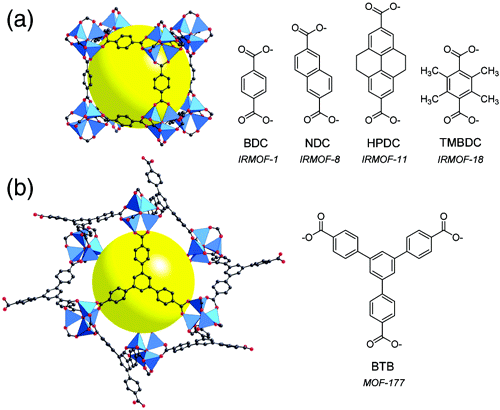
\includegraphics[width=0.65\textwidth]{figures/cited/mof-different-linker}
    \caption{Deux examples de MOFS construit avec un centre metallique zinc.
    (a) Structure de la MOF-5, avec un ligand linéaire. (b) Structure de la
    MOF-177, avec un ligand trigonal. Adapté de la référence~\cite{Rowsell2004}.}
    \label{fig:fr:mof-different-linkers}
\end{figure}

La faiblesse relative des liaisons de coordination entre les cations métalliques
et les ligands organiques est à l'origine d'une flexibilité structurelle
intrinsèque dans les MOFs, qui peut être locale ou étendue à l'ensemble du
matériau. Certain MOF, regroupés sous l'appellation \emph{"soft porous
crystals"}, réagissent à des stimuli externes comme la température, la pression,
l'adsorption de gaz ou même l'exposition à la lumière avec des modifications de
grande envergure de leur structure. Les différents modes de flexibilité pouvant
exister dans les MOFs sont représentés en figure~\ref{fig:fr:mof-flexibility}.
Si tous les MOFs peuvent présenter des déformations locales comme la rotation de
ligands, seuls les \emph{soft porous crystals} présente des déformations
globale. Par exemple, les matériaux de la famille MIL-53 présentent deux
transitions de phase, allant d'une phase à pores ouverts à une phase à pores
fermés, puis de nouveau à la phase à pores ouverts\cite{Serre2002} losque l'on
augmente de manière continue de la quantité de gaz adsorbé, donnant naissance à
une \emph{respiration} du matériau.

\begin{figure}[ht]
    \centering
    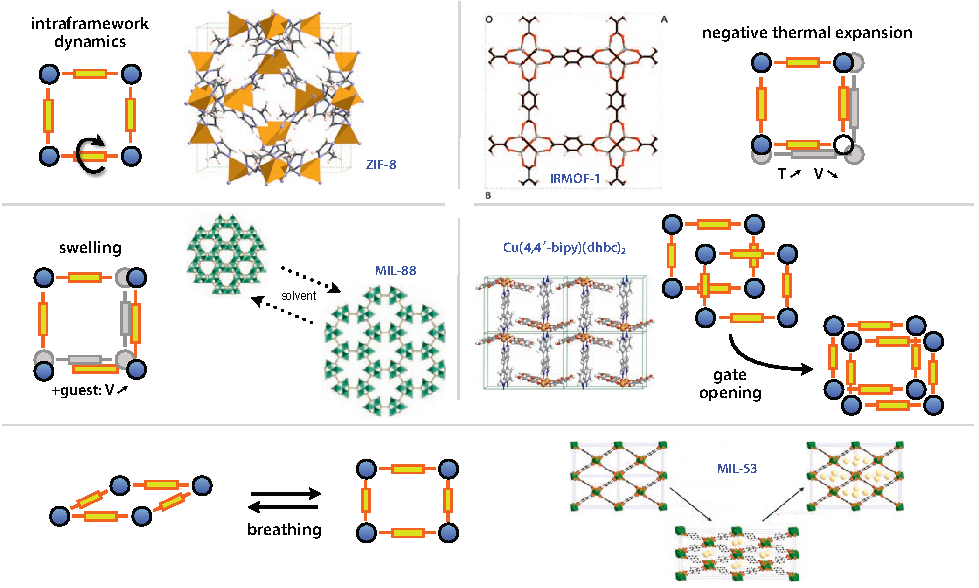
\includegraphics[width=\textwidth]{figures/cited/mof-flexibility}
    \caption{Illustration des principaux modes de flexibilité des MOFs: rotation
    de ligands, expansion thermique, gonflement, ouverture de porte et
    respiration. Image adaptée de la référence~\cite{Coudert2011}.}
    \label{fig:fr:mof-flexibility}
\end{figure}

La plupart des applications des matériaux nanoporeux, sont liées à l'entrée
d'autres espèces chimiques (en phase liquide ou gazeuse) à l'intérieur des pores
du materiau. Lorsque le fluide à l'exterieur est dans l'état gazeux, le
processus est appelé adsorption, tandis que pour les liquides, on parle
d'intrusion. Les processus d'adsorption et d'intrusion ont tous deux un effet
sur les propriétés physiques et chimiques du fluide confiné dans les nanopores.
Les fluides confinés sont généralement organisés plus régulièrement, prenant
ainsi l'aspect d'une phase solide tout en restant mobiles. L'inverse est
également vrai: la présence du fluide à l'intérieur des pores peut modifier les
propriétés et le comportement du matériau environnant. Les matériaux flexibles
sont particulièrement touchés et peuvent subir des transitions de phase induites
par l'adsorption, entraînant des phénomènes macroscopiques comme une
\emph{"ouverture de portes"} (\emph{gate-opening}), la respiration ou
l'adsorption négative de gaz. Le couplage entre l'adsorption ou l'intrusion et
les changements de structure des matériaux nanoporeux flexibles est difficile à
étudier, car il implique des équilibres de phases entre les fluides confinés et
en dans l'état standard, ainsi que l'équilibre entre différentes phases du
matériau.

Pendant ma thèse, je me suis intéressé à la simulation moléculaire de
l'adsorption et de l'intrusion de fluides dans les matériaux nanoporeux
flexibles. Les outils de simulation moléculaire peuvent accélérer le
développement de nouveaux matériaux adaptés à des applications spécifiques en
prédisant les propriétés de nouveaux matériaux avant leur synthèse, réduisant
ainsi le coût de création d'un nouveau matériau. Les propriétés qui peuvent être
étudiées et la fiabilité des prédictions correspondantes dépendent des
techniques utilisées pour modéliser les systèmes en question. Au cours de ma
thèse, j'ai utilisé plusieurs techniques à différentes échelles de temps et de
taille pour étudier l'adsorption et l'intrusion dans les matériaux poreux
flexibles, et leurs effets tant sur le fluide confiné que les matériaux. J'ai
ainsi utilisé des modèles macroscopiques basés sur la thermodynamique classique
pour l'étude de la co-adsorption des gaz, des simulations \emph{"umbrella
sampling"} pour extraire des profils d'énergie libre d'intrusion de l'eau, la
dynamique moléculaire classique et les simulation Monte-Carlo classiques pour
l'intrusion d'eau et de solutions aqueuses dans des matériaux rigides et
flexibles, et des simulations de dynamique moléculaire \abinitio pour étudier
l'organisation moléculaire des fluides dans des pores.

\newpage
\section{Séparation de gaz dans des matériaux flexibles}

\begin{figure}[h]
    \centering
    \raisebox{-0.5\height}{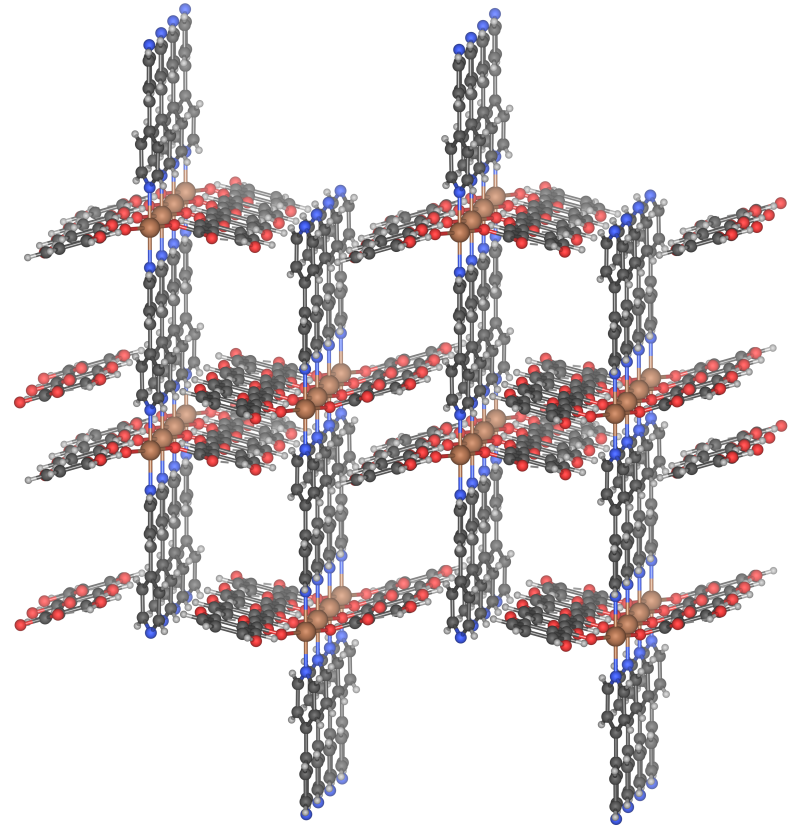
\includegraphics[width=0.35\textwidth]{figures/images/cu-dhbc-structure}}
    \hfill
    \raisebox{-0.5\height}{% GNUPLOT: LaTeX picture with Postscript
\begingroup
  \makeatletter
  \providecommand\color[2][]{%
    \GenericError{(gnuplot) \space\space\space\@spaces}{%
      Package color not loaded in conjunction with
      terminal option `colourtext'%
    }{See the gnuplot documentation for explanation.%
    }{Either use 'blacktext' in gnuplot or load the package
      color.sty in LaTeX.}%
    \renewcommand\color[2][]{}%
  }%
  \providecommand\includegraphics[2][]{%
    \GenericError{(gnuplot) \space\space\space\@spaces}{%
      Package graphicx or graphics not loaded%
    }{See the gnuplot documentation for explanation.%
    }{The gnuplot epslatex terminal needs graphicx.sty or graphics.sty.}%
    \renewcommand\includegraphics[2][]{}%
  }%
  \providecommand\rotatebox[2]{#2}%
  \@ifundefined{ifGPcolor}{%
    \newif\ifGPcolor
    \GPcolortrue
  }{}%
  \@ifundefined{ifGPblacktext}{%
    \newif\ifGPblacktext
    \GPblacktextfalse
  }{}%
  % define a \g@addto@macro without @ in the name:
  \let\gplgaddtomacro\g@addto@macro
  % define empty templates for all commands taking text:
  \gdef\gplbacktext{}%
  \gdef\gplfronttext{}%
  \makeatother
  \ifGPblacktext
    % no textcolor at all
    \def\colorrgb#1{}%
    \def\colorgray#1{}%
  \else
    % gray or color?
    \ifGPcolor
      \def\colorrgb#1{\color[rgb]{#1}}%
      \def\colorgray#1{\color[gray]{#1}}%
      \expandafter\def\csname LTw\endcsname{\color{white}}%
      \expandafter\def\csname LTb\endcsname{\color{black}}%
      \expandafter\def\csname LTa\endcsname{\color{black}}%
      \expandafter\def\csname LT0\endcsname{\color[rgb]{1,0,0}}%
      \expandafter\def\csname LT1\endcsname{\color[rgb]{0,1,0}}%
      \expandafter\def\csname LT2\endcsname{\color[rgb]{0,0,1}}%
      \expandafter\def\csname LT3\endcsname{\color[rgb]{1,0,1}}%
      \expandafter\def\csname LT4\endcsname{\color[rgb]{0,1,1}}%
      \expandafter\def\csname LT5\endcsname{\color[rgb]{1,1,0}}%
      \expandafter\def\csname LT6\endcsname{\color[rgb]{0,0,0}}%
      \expandafter\def\csname LT7\endcsname{\color[rgb]{1,0.3,0}}%
      \expandafter\def\csname LT8\endcsname{\color[rgb]{0.5,0.5,0.5}}%
    \else
      % gray
      \def\colorrgb#1{\color{black}}%
      \def\colorgray#1{\color[gray]{#1}}%
      \expandafter\def\csname LTw\endcsname{\color{white}}%
      \expandafter\def\csname LTb\endcsname{\color{black}}%
      \expandafter\def\csname LTa\endcsname{\color{black}}%
      \expandafter\def\csname LT0\endcsname{\color{black}}%
      \expandafter\def\csname LT1\endcsname{\color{black}}%
      \expandafter\def\csname LT2\endcsname{\color{black}}%
      \expandafter\def\csname LT3\endcsname{\color{black}}%
      \expandafter\def\csname LT4\endcsname{\color{black}}%
      \expandafter\def\csname LT5\endcsname{\color{black}}%
      \expandafter\def\csname LT6\endcsname{\color{black}}%
      \expandafter\def\csname LT7\endcsname{\color{black}}%
      \expandafter\def\csname LT8\endcsname{\color{black}}%
    \fi
  \fi
    \setlength{\unitlength}{0.0500bp}%
    \ifx\gptboxheight\undefined%
      \newlength{\gptboxheight}%
      \newlength{\gptboxwidth}%
      \newsavebox{\gptboxtext}%
    \fi%
    \setlength{\fboxrule}{0.5pt}%
    \setlength{\fboxsep}{1pt}%
\begin{picture}(4520.00,3400.00)%
    \gplgaddtomacro\gplbacktext{%
      \csname LTb\endcsname%%
      \put(441,595){\makebox(0,0)[r]{\strut{}$0$}}%
      \csname LTb\endcsname%%
      \put(441,1468){\makebox(0,0)[r]{\strut{}$1$}}%
      \csname LTb\endcsname%%
      \put(441,2340){\makebox(0,0)[r]{\strut{}$2$}}%
      \csname LTb\endcsname%%
      \put(441,3213){\makebox(0,0)[r]{\strut{}$3$}}%
      \csname LTb\endcsname%%
      \put(543,409){\makebox(0,0){\strut{}$0$}}%
      \csname LTb\endcsname%%
      \put(1461,409){\makebox(0,0){\strut{}$20$}}%
      \csname LTb\endcsname%%
      \put(2378,409){\makebox(0,0){\strut{}$40$}}%
      \csname LTb\endcsname%%
      \put(3296,409){\makebox(0,0){\strut{}$60$}}%
      \csname LTb\endcsname%%
      \put(4213,409){\makebox(0,0){\strut{}$80$}}%
    }%
    \gplgaddtomacro\gplfronttext{%
      \csname LTb\endcsname%%
      \put(153,1904){\rotatebox{-270}{\makebox(0,0){\strut{}uptake / (mol/mol)}}}%
      \csname LTb\endcsname%%
      \put(2378,130){\makebox(0,0){\strut{}pressure / atm}}%
      \csname LTb\endcsname%%
      \put(3425,1271){\makebox(0,0)[r]{\strut{}CH$_4$}}%
      \csname LTb\endcsname%%
      \put(3425,1030){\makebox(0,0)[r]{\strut{}CO$_2$}}%
      \csname LTb\endcsname%%
      \put(3425,789){\makebox(0,0)[r]{\strut{}O$_2$}}%
    }%
    \gplbacktext
    \put(0,0){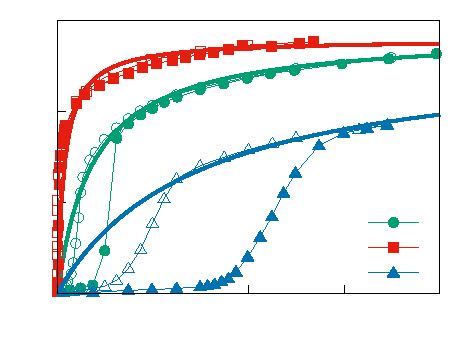
\includegraphics{cu-dhbc}}%
    \gplfronttext
  \end{picture}%
\endgroup
}
    \vskip-1em
    \caption{(gauche) Structure de \Cudhbc. (droite) Isothermes d'adsorption à
    \SI{298}{K} dans \Cudhbc pour différents gaz.  L'adsorption est représenté
    en symboles plein, la desorption en symboles creux et les lignes épaisses r
    représentent l'ajustement des données sur un modèle de Langmuir. Les données
    expérimentale ont été publiées par \citeauthor{Kitaura2003}\cite{Kitaura2003}}
    \label{fig:fr:cu-dhbc}
\end{figure}

La séparation de gaz est une étape importante dans de multiples procédés
industriels, allant de séparation des hydrocarbures dans la chimie du pétrole, à
la séparation et stockage du \ce{CO2} ou l'extraction d'oxygène dans l'air. Les
deux principales méthodes utilisées pour la séparation des gaz sont la
distillation cryogénique, principalement utilisée pour la séparation de l'air,
et l'adsorption différentielle. Les procédés de séparation des gaz basés sur
l'adsorption sont très polyvalents grâce au large choix de matériaux disponibles
--- et de la possibilité d'adapter l'adsorbant à un système de gaz spécifique.
Pour choisir un adsorbant et la taille d'une unité de production pour la
séparation d'un mélange gazeux, une bonne connaissance des propriétés de
co-adsorption de ces gaz est nécessaire.

La caractérisation expérimentale de la co-adsorption est en général longue et
couteuse, à cause du grand nombre de paramètres à faire varier. Pour un mélange
ternaire, par exemple, il y a quatre variables indépendantes: la température, la
pression totale et deux variables supplémentaires pour la composition du mélange.
Ce coût important est à l'origine de plusieurs modèles théoriques permettant de
prédire la co-adsorption à partir de données d'adsorption de corps purs. La
méthode la plus couramment utilisée sur la théorie des solutions adsorbée idéale
(\emph{Ideal Adsorbed Solution Theory}, IAST)\cite{Myers1965}, qui est robuste
et relativement simple à mettre en œuvre.

En pratique, l'utilisation de la méthode IAST revient à travailler dans
l'ensemble thermodynamique grand-canonique, et à considérer la matrice
d'adsorption comme étant rigide. Pour pouvoir décrire la flexibilité des
matériaux lors de l'adsorption, il faut à la place utiliser l'ensemble
osmotique. Cet ensemble osmotique est à la base de la méthode OFAST
(\emph{Osmotic Framework Adsorbed Solution Theory}) développée dans le
groupe\cite{Coudert2010, Ortiz2011}. Pour une description plus en détail de ces
méthodes, je renvoie le lecteur vers le chapitre~\ref{sec:macroscopic} de ce
manuscrit, ou à l'article correspondant~\cite{Fraux2018}.

Durant ma thèse, j'ai utilisé à la fois IAST et OFAST pour calculer la
sélectivité d'adsorption dans les MOFs \Cudhbc et \RPMZn, et démontrer par un
exemple l'inadéquation d'IAST lorsque les structures adsorbantes sont flexibles.
Je vais rappeler rapidement ici les résultat obtenus dans le cas de \Cudhbc.
L'adsorption dans ce matériau, présenté en figure~\ref{fig:fr:cu-dhbc}, est
représentatif du phénomène d'ouverture de portes: en dessus d'une pression
"d'ouverture", aucune molécule de gaz n'entre dans la structure, et au delà de
cette pression l'adsorption se produit normalement. La selectivité prédite à
partir de ces isothermes d'adsorption par IAST et OFAST est présentée en
figure~\ref{fig:fr:cu-dhbc:iast-ofast:selectivity}.

\begin{figure}[t]
    \centering
    % GNUPLOT: LaTeX picture with Postscript
\begingroup
  \makeatletter
  \providecommand\color[2][]{%
    \GenericError{(gnuplot) \space\space\space\@spaces}{%
      Package color not loaded in conjunction with
      terminal option `colourtext'%
    }{See the gnuplot documentation for explanation.%
    }{Either use 'blacktext' in gnuplot or load the package
      color.sty in LaTeX.}%
    \renewcommand\color[2][]{}%
  }%
  \providecommand\includegraphics[2][]{%
    \GenericError{(gnuplot) \space\space\space\@spaces}{%
      Package graphicx or graphics not loaded%
    }{See the gnuplot documentation for explanation.%
    }{The gnuplot epslatex terminal needs graphicx.sty or graphics.sty.}%
    \renewcommand\includegraphics[2][]{}%
  }%
  \providecommand\rotatebox[2]{#2}%
  \@ifundefined{ifGPcolor}{%
    \newif\ifGPcolor
    \GPcolortrue
  }{}%
  \@ifundefined{ifGPblacktext}{%
    \newif\ifGPblacktext
    \GPblacktextfalse
  }{}%
  % define a \g@addto@macro without @ in the name:
  \let\gplgaddtomacro\g@addto@macro
  % define empty templates for all commands taking text:
  \gdef\gplbacktext{}%
  \gdef\gplfronttext{}%
  \makeatother
  \ifGPblacktext
    % no textcolor at all
    \def\colorrgb#1{}%
    \def\colorgray#1{}%
  \else
    % gray or color?
    \ifGPcolor
      \def\colorrgb#1{\color[rgb]{#1}}%
      \def\colorgray#1{\color[gray]{#1}}%
      \expandafter\def\csname LTw\endcsname{\color{white}}%
      \expandafter\def\csname LTb\endcsname{\color{black}}%
      \expandafter\def\csname LTa\endcsname{\color{black}}%
      \expandafter\def\csname LT0\endcsname{\color[rgb]{1,0,0}}%
      \expandafter\def\csname LT1\endcsname{\color[rgb]{0,1,0}}%
      \expandafter\def\csname LT2\endcsname{\color[rgb]{0,0,1}}%
      \expandafter\def\csname LT3\endcsname{\color[rgb]{1,0,1}}%
      \expandafter\def\csname LT4\endcsname{\color[rgb]{0,1,1}}%
      \expandafter\def\csname LT5\endcsname{\color[rgb]{1,1,0}}%
      \expandafter\def\csname LT6\endcsname{\color[rgb]{0,0,0}}%
      \expandafter\def\csname LT7\endcsname{\color[rgb]{1,0.3,0}}%
      \expandafter\def\csname LT8\endcsname{\color[rgb]{0.5,0.5,0.5}}%
    \else
      % gray
      \def\colorrgb#1{\color{black}}%
      \def\colorgray#1{\color[gray]{#1}}%
      \expandafter\def\csname LTw\endcsname{\color{white}}%
      \expandafter\def\csname LTb\endcsname{\color{black}}%
      \expandafter\def\csname LTa\endcsname{\color{black}}%
      \expandafter\def\csname LT0\endcsname{\color{black}}%
      \expandafter\def\csname LT1\endcsname{\color{black}}%
      \expandafter\def\csname LT2\endcsname{\color{black}}%
      \expandafter\def\csname LT3\endcsname{\color{black}}%
      \expandafter\def\csname LT4\endcsname{\color{black}}%
      \expandafter\def\csname LT5\endcsname{\color{black}}%
      \expandafter\def\csname LT6\endcsname{\color{black}}%
      \expandafter\def\csname LT7\endcsname{\color{black}}%
      \expandafter\def\csname LT8\endcsname{\color{black}}%
    \fi
  \fi
    \setlength{\unitlength}{0.0500bp}%
    \ifx\gptboxheight\undefined%
      \newlength{\gptboxheight}%
      \newlength{\gptboxwidth}%
      \newsavebox{\gptboxtext}%
    \fi%
    \setlength{\fboxrule}{0.5pt}%
    \setlength{\fboxsep}{1pt}%
\begin{picture}(7360.00,6800.00)%
    \gplgaddtomacro\gplbacktext{%
      \csname LTb\endcsname%%
      \put(747,4971){\makebox(0,0)[r]{\strut{}$0$}}%
      \csname LTb\endcsname%%
      \put(747,5628){\makebox(0,0)[r]{\strut{}$1000$}}%
      \csname LTb\endcsname%%
      \put(747,6285){\makebox(0,0)[r]{\strut{}$2000$}}%
      \csname LTb\endcsname%%
      \put(849,4719){\makebox(0,0){\strut{}$0$}}%
      \csname LTb\endcsname%%
      \put(1480,4719){\makebox(0,0){\strut{}$20$}}%
      \csname LTb\endcsname%%
      \put(2111,4719){\makebox(0,0){\strut{}$40$}}%
      \csname LTb\endcsname%%
      \put(2742,4719){\makebox(0,0){\strut{}$60$}}%
      \csname LTb\endcsname%%
      \put(3373,4719){\makebox(0,0){\strut{}$80$}}%
    }%
    \gplgaddtomacro\gplfronttext{%
      \csname LTb\endcsname%%
      \put(153,5759){\rotatebox{-270}{\makebox(0,0){\strut{}\ce{CO2} / \ce{O2} selectivity}}}%
      \csname LTb\endcsname%%
      \put(2585,6418){\makebox(0,0)[r]{\strut{}$y_{\ce{CO2}} = 0.1$}}%
      \csname LTb\endcsname%%
      \put(2585,6177){\makebox(0,0)[r]{\strut{}$y_{\ce{CO2}} = 0.5$}}%
      \csname LTb\endcsname%%
      \put(2585,5936){\makebox(0,0)[r]{\strut{}$y_{\ce{CO2}} = 0.9$}}%
    }%
    \gplgaddtomacro\gplbacktext{%
      \csname LTb\endcsname%%
      \put(4241,4905){\makebox(0,0)[r]{\strut{}$1$}}%
      \csname LTb\endcsname%%
      \put(4241,5343){\makebox(0,0)[r]{\strut{}$10$}}%
      \csname LTb\endcsname%%
      \put(4241,5780){\makebox(0,0)[r]{\strut{}$100$}}%
      \csname LTb\endcsname%%
      \put(4241,6218){\makebox(0,0)[r]{\strut{}$1000$}}%
      \csname LTb\endcsname%%
      \put(4343,4719){\makebox(0,0){\strut{}$0$}}%
      \csname LTb\endcsname%%
      \put(5021,4719){\makebox(0,0){\strut{}$20$}}%
      \csname LTb\endcsname%%
      \put(5698,4719){\makebox(0,0){\strut{}$40$}}%
      \csname LTb\endcsname%%
      \put(6376,4719){\makebox(0,0){\strut{}$60$}}%
      \csname LTb\endcsname%%
      \put(7053,4719){\makebox(0,0){\strut{}$80$}}%
    }%
    \gplgaddtomacro\gplfronttext{%
    }%
    \gplgaddtomacro\gplbacktext{%
      \csname LTb\endcsname%%
      \put(543,2719){\makebox(0,0)[r]{\strut{}$0$}}%
      \csname LTb\endcsname%%
      \put(543,3533){\makebox(0,0)[r]{\strut{}$5$}}%
      \csname LTb\endcsname%%
      \put(543,4347){\makebox(0,0)[r]{\strut{}$10$}}%
      \csname LTb\endcsname%%
      \put(645,2452){\makebox(0,0){\strut{}$0$}}%
      \csname LTb\endcsname%%
      \put(1327,2452){\makebox(0,0){\strut{}$20$}}%
      \csname LTb\endcsname%%
      \put(2009,2452){\makebox(0,0){\strut{}$40$}}%
      \csname LTb\endcsname%%
      \put(2691,2452){\makebox(0,0){\strut{}$60$}}%
      \csname LTb\endcsname%%
      \put(3373,2452){\makebox(0,0){\strut{}$80$}}%
    }%
    \gplgaddtomacro\gplfronttext{%
      \csname LTb\endcsname%%
      \put(153,3492){\rotatebox{-270}{\makebox(0,0){\strut{}\ce{CH4} / \ce{O2} selectivity}}}%
    }%
    \gplgaddtomacro\gplbacktext{%
      \csname LTb\endcsname%%
      \put(4037,2638){\makebox(0,0)[r]{\strut{}$1$}}%
      \csname LTb\endcsname%%
      \put(4037,4347){\makebox(0,0)[r]{\strut{}$10$}}%
      \csname LTb\endcsname%%
      \put(4139,2452){\makebox(0,0){\strut{}$0$}}%
      \csname LTb\endcsname%%
      \put(4868,2452){\makebox(0,0){\strut{}$20$}}%
      \csname LTb\endcsname%%
      \put(5596,2452){\makebox(0,0){\strut{}$40$}}%
      \csname LTb\endcsname%%
      \put(6325,2452){\makebox(0,0){\strut{}$60$}}%
      \csname LTb\endcsname%%
      \put(7053,2452){\makebox(0,0){\strut{}$80$}}%
    }%
    \gplgaddtomacro\gplfronttext{%
    }%
    \gplgaddtomacro\gplbacktext{%
      \csname LTb\endcsname%%
      \put(645,595){\makebox(0,0)[r]{\strut{}$0$}}%
      \csname LTb\endcsname%%
      \put(645,1338){\makebox(0,0)[r]{\strut{}$0.5$}}%
      \csname LTb\endcsname%%
      \put(645,2080){\makebox(0,0)[r]{\strut{}$1$}}%
      \csname LTb\endcsname%%
      \put(747,409){\makebox(0,0){\strut{}$0$}}%
      \csname LTb\endcsname%%
      \put(1404,409){\makebox(0,0){\strut{}$20$}}%
      \csname LTb\endcsname%%
      \put(2060,409){\makebox(0,0){\strut{}$40$}}%
      \csname LTb\endcsname%%
      \put(2717,409){\makebox(0,0){\strut{}$60$}}%
      \csname LTb\endcsname%%
      \put(3373,409){\makebox(0,0){\strut{}$80$}}%
    }%
    \gplgaddtomacro\gplfronttext{%
      \csname LTb\endcsname%%
      \put(153,1337){\rotatebox{-270}{\makebox(0,0){\strut{}\ce{CH4} / \ce{CO2} selectivity}}}%
      \csname LTb\endcsname%%
      \put(2060,130){\makebox(0,0){\strut{}pressure / atm}}%
    }%
    \gplgaddtomacro\gplbacktext{%
      \csname LTb\endcsname%%
      \put(4241,595){\makebox(0,0)[r]{\strut{}$0.01$}}%
      \csname LTb\endcsname%%
      \put(4241,1338){\makebox(0,0)[r]{\strut{}$0.1$}}%
      \csname LTb\endcsname%%
      \put(4241,2080){\makebox(0,0)[r]{\strut{}$1$}}%
      \csname LTb\endcsname%%
      \put(4343,409){\makebox(0,0){\strut{}$0$}}%
      \csname LTb\endcsname%%
      \put(5021,409){\makebox(0,0){\strut{}$20$}}%
      \csname LTb\endcsname%%
      \put(5698,409){\makebox(0,0){\strut{}$40$}}%
      \csname LTb\endcsname%%
      \put(6376,409){\makebox(0,0){\strut{}$60$}}%
      \csname LTb\endcsname%%
      \put(7053,409){\makebox(0,0){\strut{}$80$}}%
    }%
    \gplgaddtomacro\gplfronttext{%
      \csname LTb\endcsname%%
      \put(5698,130){\makebox(0,0){\strut{}pressure / atm}}%
    }%
    \gplbacktext
    \put(0,0){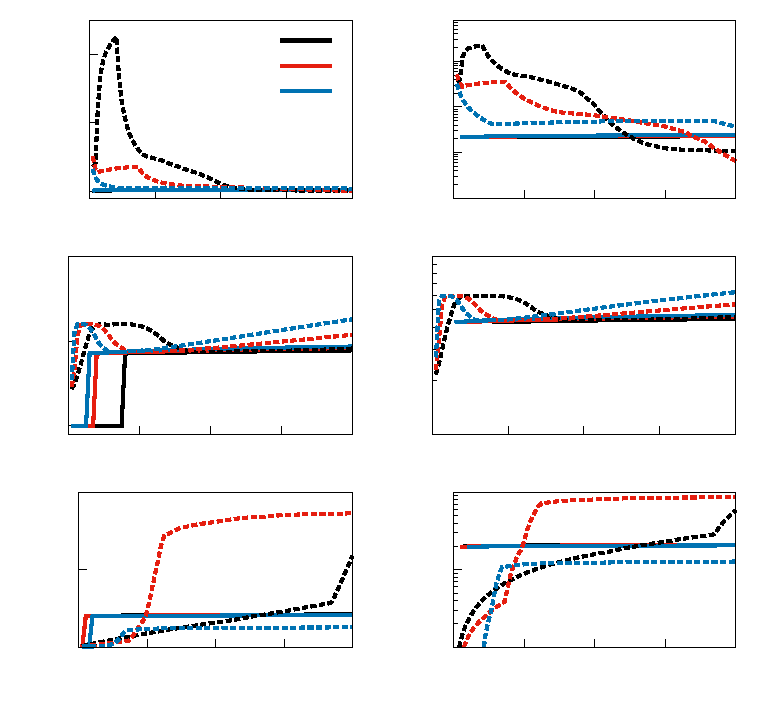
\includegraphics{cu-dhbc-selectivities}}%
    \gplfronttext
  \end{picture}%
\endgroup

    \vskip-3em
    \caption{Comparaison de la sélectivité prédite par la méthodes IAST (lignes
    pointillées) ou OFAST (lignes pleines) pour les couples \ce{CO2}/\ce{O2}
    (haut); \ce{CH4}/\ce{O2} (milieu) et \ce{CH4}/\ce{CO2} (bas) dans \Cudhbc;
    en échelle linéaire (gauche) et logarithmique (droite).}
    \label{fig:fr:cu-dhbc:iast-ofast:selectivity}
\end{figure}

La sélectivité d'adsorption calculée avec OFAST se comporte comme attendu: à
basse pression, les pores sont fermés et aucun gaz n'entre dans la structure.
Ensuite, à une pression dépendant de la composition de la phase gazeuse,
l'ouverture de porte se produit. Pour les pressions plus importantes, le
matériau est sous sa forme ouverte, et la valeur de sélectivité dépend de la
différence en capacité d'absorption entre les deux gaz, environ 20 pour les
mélanges \ce{CO2}/\ce{O2} et 4 pour les mélanges \ce{CH4}/\ce{O2}.

Au contraire, les sélectivités calculées par la méthode IAST sont clairement non
physiques. Toutes les courbes de sélectivité présentent un maximum dans la plage
de pression où se produit l'ouverture de la structure, avec des sélectivités qui
peuvent être plusieurs ordres de grandeur trop élevées, par exemple 2 000 au
lieu de 20 pour \ce{CO2}/\ce{O2}. Même loin de la pression de transition, les
sélectivités prédites par IAST ne reproduisent pas celles calculées avec OFAST,
le comportement incorrect à basse pression affectant directement les calculs
au-delà. J'ai donc pu confirmer par une étude quantitative que IAST n'est pas
adapté à l'adsorption dans les matériaux flexibles nanoporeux.

\section{Adsorption de \ce{N2} dans la \ZIF8}

\begin{figure}[ht]
    \centering
    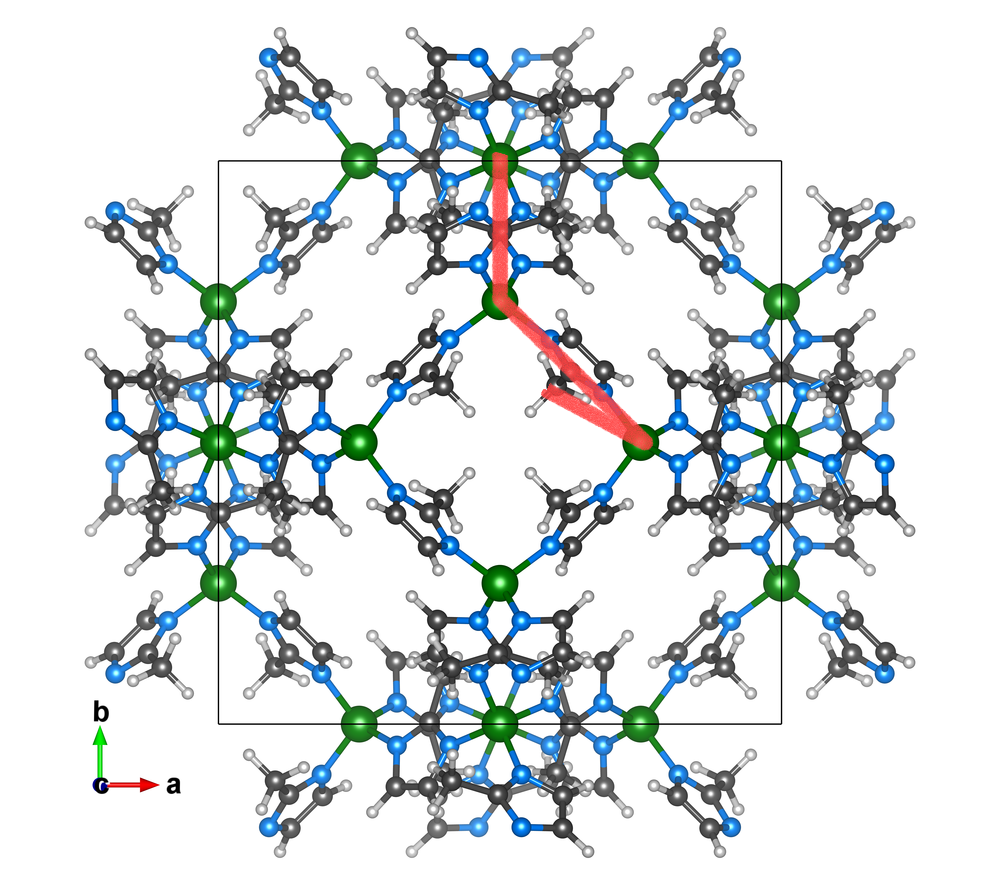
\includegraphics[width=0.45\textwidth]{figures/images/swing-angle}
    \hfill
    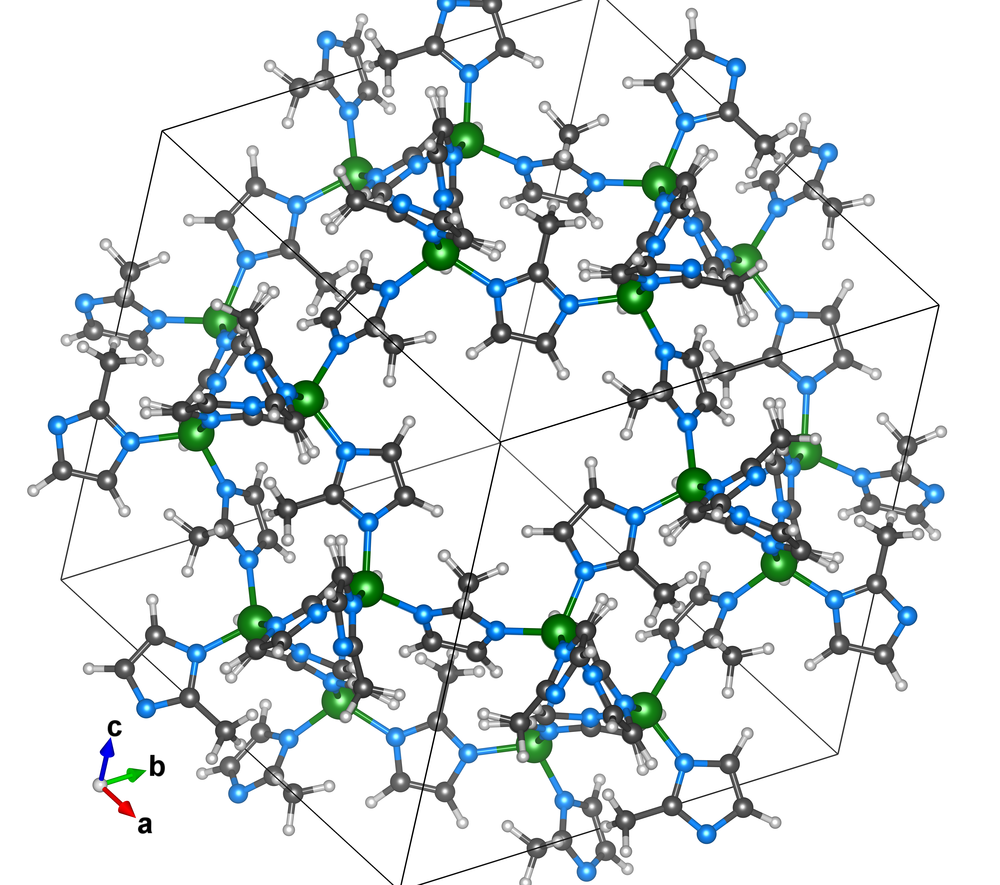
\includegraphics[width=0.45\textwidth]{figures/images/ZIF8-111}
    \caption{Structure of the methyl-imidazolate \ZIF8. On the left, the
    front-most opening is the 4-member ring window (the structure is represented
    along the 001 axis); and on the right the front-most opening is the 6-member
    ring window (the structure is represented along the 111 axis). The atomic
    color code is green for zinc, blue for nitrogen, gray for carbon and white
    for hydrogen. The red line connects the atoms of the "swing"
    \ce{Zn-Zn-Zn-X} dihedral angle.}
    \label{fig:fr:zif8-ch3:structure}
\end{figure}

\ref{fig:zif8x:isotherms}

\begin{figure}[ht]
    \centering
    % GNUPLOT: LaTeX picture with Postscript
\begingroup
  \makeatletter
  \providecommand\color[2][]{%
    \GenericError{(gnuplot) \space\space\space\@spaces}{%
      Package color not loaded in conjunction with
      terminal option `colourtext'%
    }{See the gnuplot documentation for explanation.%
    }{Either use 'blacktext' in gnuplot or load the package
      color.sty in LaTeX.}%
    \renewcommand\color[2][]{}%
  }%
  \providecommand\includegraphics[2][]{%
    \GenericError{(gnuplot) \space\space\space\@spaces}{%
      Package graphicx or graphics not loaded%
    }{See the gnuplot documentation for explanation.%
    }{The gnuplot epslatex terminal needs graphicx.sty or graphics.sty.}%
    \renewcommand\includegraphics[2][]{}%
  }%
  \providecommand\rotatebox[2]{#2}%
  \@ifundefined{ifGPcolor}{%
    \newif\ifGPcolor
    \GPcolortrue
  }{}%
  \@ifundefined{ifGPblacktext}{%
    \newif\ifGPblacktext
    \GPblacktextfalse
  }{}%
  % define a \g@addto@macro without @ in the name:
  \let\gplgaddtomacro\g@addto@macro
  % define empty templates for all commands taking text:
  \gdef\gplbacktext{}%
  \gdef\gplfronttext{}%
  \makeatother
  \ifGPblacktext
    % no textcolor at all
    \def\colorrgb#1{}%
    \def\colorgray#1{}%
  \else
    % gray or color?
    \ifGPcolor
      \def\colorrgb#1{\color[rgb]{#1}}%
      \def\colorgray#1{\color[gray]{#1}}%
      \expandafter\def\csname LTw\endcsname{\color{white}}%
      \expandafter\def\csname LTb\endcsname{\color{black}}%
      \expandafter\def\csname LTa\endcsname{\color{black}}%
      \expandafter\def\csname LT0\endcsname{\color[rgb]{1,0,0}}%
      \expandafter\def\csname LT1\endcsname{\color[rgb]{0,1,0}}%
      \expandafter\def\csname LT2\endcsname{\color[rgb]{0,0,1}}%
      \expandafter\def\csname LT3\endcsname{\color[rgb]{1,0,1}}%
      \expandafter\def\csname LT4\endcsname{\color[rgb]{0,1,1}}%
      \expandafter\def\csname LT5\endcsname{\color[rgb]{1,1,0}}%
      \expandafter\def\csname LT6\endcsname{\color[rgb]{0,0,0}}%
      \expandafter\def\csname LT7\endcsname{\color[rgb]{1,0.3,0}}%
      \expandafter\def\csname LT8\endcsname{\color[rgb]{0.5,0.5,0.5}}%
    \else
      % gray
      \def\colorrgb#1{\color{black}}%
      \def\colorgray#1{\color[gray]{#1}}%
      \expandafter\def\csname LTw\endcsname{\color{white}}%
      \expandafter\def\csname LTb\endcsname{\color{black}}%
      \expandafter\def\csname LTa\endcsname{\color{black}}%
      \expandafter\def\csname LT0\endcsname{\color{black}}%
      \expandafter\def\csname LT1\endcsname{\color{black}}%
      \expandafter\def\csname LT2\endcsname{\color{black}}%
      \expandafter\def\csname LT3\endcsname{\color{black}}%
      \expandafter\def\csname LT4\endcsname{\color{black}}%
      \expandafter\def\csname LT5\endcsname{\color{black}}%
      \expandafter\def\csname LT6\endcsname{\color{black}}%
      \expandafter\def\csname LT7\endcsname{\color{black}}%
      \expandafter\def\csname LT8\endcsname{\color{black}}%
    \fi
  \fi
    \setlength{\unitlength}{0.0500bp}%
    \ifx\gptboxheight\undefined%
      \newlength{\gptboxheight}%
      \newlength{\gptboxwidth}%
      \newsavebox{\gptboxtext}%
    \fi%
    \setlength{\fboxrule}{0.5pt}%
    \setlength{\fboxsep}{1pt}%
\begin{picture}(7760.00,3100.00)%
    \gplgaddtomacro\gplbacktext{%
      \csname LTb\endcsname%%
      \put(212,341){\makebox(0,0){\strut{}$0$}}%
      \csname LTb\endcsname%%
      \put(636,341){\makebox(0,0){\strut{}$10$}}%
      \csname LTb\endcsname%%
      \put(1060,341){\makebox(0,0){\strut{}$20$}}%
      \csname LTb\endcsname%%
      \put(1483,341){\makebox(0,0){\strut{}$30$}}%
      \csname LTb\endcsname%%
      \put(1907,341){\makebox(0,0){\strut{}$40$}}%
      \csname LTb\endcsname%%
      \put(2331,341){\makebox(0,0){\strut{}$50$}}%
    }%
    \gplgaddtomacro\gplfronttext{%
      \csname LTb\endcsname%%
      \put(1271,109){\makebox(0,0){\strut{}$\phi$ (°)}}%
      \csname LTb\endcsname%%
      \put(1271,2867){\makebox(0,0){\strut{}\ZIFCH3}}%
      \csname LTb\endcsname%%
      \put(1759,2494){\makebox(0,0)[r]{\strut{}\scriptsize 0 \ce{N2}}}%
      \csname LTb\endcsname%%
      \put(1759,2339){\makebox(0,0)[r]{\strut{}\scriptsize 10 \ce{N2}}}%
      \csname LTb\endcsname%%
      \put(1759,2184){\makebox(0,0)[r]{\strut{}\scriptsize 25 \ce{N2}}}%
      \csname LTb\endcsname%%
      \put(1759,2029){\makebox(0,0)[r]{\strut{}\scriptsize 40 \ce{N2}}}%
      \csname LTb\endcsname%%
      \put(1759,1874){\makebox(0,0)[r]{\strut{}\scriptsize 50 \ce{N2}}}%
    }%
    \gplgaddtomacro\gplbacktext{%
      \csname LTb\endcsname%%
      \put(2628,341){\makebox(0,0){\strut{}$0$}}%
      \csname LTb\endcsname%%
      \put(3086,341){\makebox(0,0){\strut{}$10$}}%
      \csname LTb\endcsname%%
      \put(3544,341){\makebox(0,0){\strut{}$20$}}%
      \csname LTb\endcsname%%
      \put(4001,341){\makebox(0,0){\strut{}$30$}}%
      \csname LTb\endcsname%%
      \put(4459,341){\makebox(0,0){\strut{}$40$}}%
      \csname LTb\endcsname%%
      \put(4917,341){\makebox(0,0){\strut{}$50$}}%
    }%
    \gplgaddtomacro\gplfronttext{%
      \csname LTb\endcsname%%
      \put(3772,109){\makebox(0,0){\strut{}$\phi$ (°)}}%
      \csname LTb\endcsname%%
      \put(3772,2867){\makebox(0,0){\strut{}\ZIFCl}}%
      \csname LTb\endcsname%%
      \put(4345,2494){\makebox(0,0)[r]{\strut{}\scriptsize 0 \ce{N2}}}%
      \csname LTb\endcsname%%
      \put(4345,2339){\makebox(0,0)[r]{\strut{}\scriptsize 10 \ce{N2}}}%
      \csname LTb\endcsname%%
      \put(4345,2184){\makebox(0,0)[r]{\strut{}\scriptsize 25 \ce{N2}}}%
      \csname LTb\endcsname%%
      \put(4345,2029){\makebox(0,0)[r]{\strut{}\scriptsize 40 \ce{N2}}}%
      \csname LTb\endcsname%%
      \put(4345,1874){\makebox(0,0)[r]{\strut{}\scriptsize 50 \ce{N2}}}%
    }%
    \gplgaddtomacro\gplbacktext{%
      \csname LTb\endcsname%%
      \put(5215,341){\makebox(0,0){\strut{}$0$}}%
      \csname LTb\endcsname%%
      \put(5673,341){\makebox(0,0){\strut{}$10$}}%
      \csname LTb\endcsname%%
      \put(6131,341){\makebox(0,0){\strut{}$20$}}%
      \csname LTb\endcsname%%
      \put(6588,341){\makebox(0,0){\strut{}$30$}}%
      \csname LTb\endcsname%%
      \put(7046,341){\makebox(0,0){\strut{}$40$}}%
      \csname LTb\endcsname%%
      \put(7504,341){\makebox(0,0){\strut{}$50$}}%
    }%
    \gplgaddtomacro\gplfronttext{%
      \csname LTb\endcsname%%
      \put(6359,109){\makebox(0,0){\strut{}$\phi$ (°)}}%
      \csname LTb\endcsname%%
      \put(6359,2867){\makebox(0,0){\strut{}\ZIFBr}}%
      \csname LTb\endcsname%%
      \put(6932,2494){\makebox(0,0)[r]{\strut{}\scriptsize 0 \ce{N2}}}%
      \csname LTb\endcsname%%
      \put(6932,2339){\makebox(0,0)[r]{\strut{}\scriptsize 8 \ce{N2}}}%
      \csname LTb\endcsname%%
      \put(6932,2184){\makebox(0,0)[r]{\strut{}\scriptsize 20 \ce{N2}}}%
      \csname LTb\endcsname%%
      \put(6932,2029){\makebox(0,0)[r]{\strut{}\scriptsize 40 \ce{N2}}}%
      \csname LTb\endcsname%%
      \put(6932,1874){\makebox(0,0)[r]{\strut{}\scriptsize 50 \ce{N2}}}%
    }%
    \gplbacktext
    \put(0,0){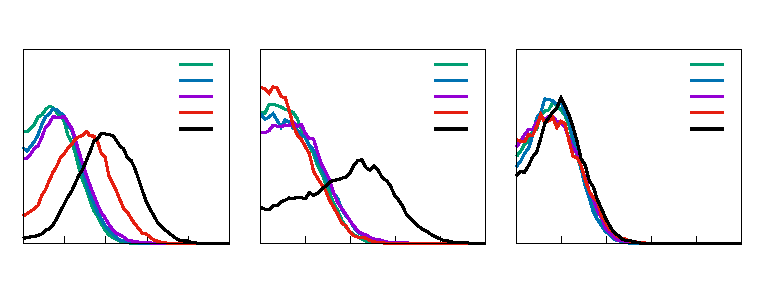
\includegraphics{zif8x-dihedrals}}%
    \gplfronttext
  \end{picture}%
\endgroup

    \caption{Distribution of linker swing angle (\ce{Zn-Zn-Zn-X} dihedral angle,
    where \ce{X} stands for \ce{CH3}, \ce{Cl} or \ce{Br} for \ZIFCH3, \ZIFCl or
    \ZIFBr, respectively) at various values of nitrogen loading.}
    \label{fig:fr:zif8x:dihedrals}
\end{figure}

\begin{figure}[ht]
    \centering
    % GNUPLOT: LaTeX picture with Postscript
\begingroup
  \makeatletter
  \providecommand\color[2][]{%
    \GenericError{(gnuplot) \space\space\space\@spaces}{%
      Package color not loaded in conjunction with
      terminal option `colourtext'%
    }{See the gnuplot documentation for explanation.%
    }{Either use 'blacktext' in gnuplot or load the package
      color.sty in LaTeX.}%
    \renewcommand\color[2][]{}%
  }%
  \providecommand\includegraphics[2][]{%
    \GenericError{(gnuplot) \space\space\space\@spaces}{%
      Package graphicx or graphics not loaded%
    }{See the gnuplot documentation for explanation.%
    }{The gnuplot epslatex terminal needs graphicx.sty or graphics.sty.}%
    \renewcommand\includegraphics[2][]{}%
  }%
  \providecommand\rotatebox[2]{#2}%
  \@ifundefined{ifGPcolor}{%
    \newif\ifGPcolor
    \GPcolortrue
  }{}%
  \@ifundefined{ifGPblacktext}{%
    \newif\ifGPblacktext
    \GPblacktextfalse
  }{}%
  % define a \g@addto@macro without @ in the name:
  \let\gplgaddtomacro\g@addto@macro
  % define empty templates for all commands taking text:
  \gdef\gplbacktext{}%
  \gdef\gplfronttext{}%
  \makeatother
  \ifGPblacktext
    % no textcolor at all
    \def\colorrgb#1{}%
    \def\colorgray#1{}%
  \else
    % gray or color?
    \ifGPcolor
      \def\colorrgb#1{\color[rgb]{#1}}%
      \def\colorgray#1{\color[gray]{#1}}%
      \expandafter\def\csname LTw\endcsname{\color{white}}%
      \expandafter\def\csname LTb\endcsname{\color{black}}%
      \expandafter\def\csname LTa\endcsname{\color{black}}%
      \expandafter\def\csname LT0\endcsname{\color[rgb]{1,0,0}}%
      \expandafter\def\csname LT1\endcsname{\color[rgb]{0,1,0}}%
      \expandafter\def\csname LT2\endcsname{\color[rgb]{0,0,1}}%
      \expandafter\def\csname LT3\endcsname{\color[rgb]{1,0,1}}%
      \expandafter\def\csname LT4\endcsname{\color[rgb]{0,1,1}}%
      \expandafter\def\csname LT5\endcsname{\color[rgb]{1,1,0}}%
      \expandafter\def\csname LT6\endcsname{\color[rgb]{0,0,0}}%
      \expandafter\def\csname LT7\endcsname{\color[rgb]{1,0.3,0}}%
      \expandafter\def\csname LT8\endcsname{\color[rgb]{0.5,0.5,0.5}}%
    \else
      % gray
      \def\colorrgb#1{\color{black}}%
      \def\colorgray#1{\color[gray]{#1}}%
      \expandafter\def\csname LTw\endcsname{\color{white}}%
      \expandafter\def\csname LTb\endcsname{\color{black}}%
      \expandafter\def\csname LTa\endcsname{\color{black}}%
      \expandafter\def\csname LT0\endcsname{\color{black}}%
      \expandafter\def\csname LT1\endcsname{\color{black}}%
      \expandafter\def\csname LT2\endcsname{\color{black}}%
      \expandafter\def\csname LT3\endcsname{\color{black}}%
      \expandafter\def\csname LT4\endcsname{\color{black}}%
      \expandafter\def\csname LT5\endcsname{\color{black}}%
      \expandafter\def\csname LT6\endcsname{\color{black}}%
      \expandafter\def\csname LT7\endcsname{\color{black}}%
      \expandafter\def\csname LT8\endcsname{\color{black}}%
    \fi
  \fi
    \setlength{\unitlength}{0.0500bp}%
    \ifx\gptboxheight\undefined%
      \newlength{\gptboxheight}%
      \newlength{\gptboxwidth}%
      \newsavebox{\gptboxtext}%
    \fi%
    \setlength{\fboxrule}{0.5pt}%
    \setlength{\fboxsep}{1pt}%
\begin{picture}(7360.00,7360.00)%
    \gplgaddtomacro\gplbacktext{%
    }%
    \gplgaddtomacro\gplfronttext{%
      \csname LTb\endcsname%%
      \put(919,7250){\makebox(0,0){\strut{}\small 10 \ce{N2} $\in$ \ZIFCH3}}%
    }%
    \gplgaddtomacro\gplbacktext{%
    }%
    \gplgaddtomacro\gplfronttext{%
      \csname LTb\endcsname%%
      \put(2759,7250){\makebox(0,0){\strut{}\small 25 \ce{N2} $\in$ \ZIFCH3}}%
    }%
    \gplgaddtomacro\gplbacktext{%
    }%
    \gplgaddtomacro\gplfronttext{%
      \csname LTb\endcsname%%
      \put(4599,7250){\makebox(0,0){\strut{}\small 40 \ce{N2} $\in$ \ZIFCH3}}%
    }%
    \gplgaddtomacro\gplbacktext{%
    }%
    \gplgaddtomacro\gplfronttext{%
      \csname LTb\endcsname%%
      \put(6439,7250){\makebox(0,0){\strut{}\small 50 \ce{N2} $\in$ \ZIFCH3}}%
    }%
    \gplgaddtomacro\gplbacktext{%
    }%
    \gplgaddtomacro\gplfronttext{%
      \csname LTb\endcsname%%
      \put(919,4797){\makebox(0,0){\strut{}\small 10 \ce{N2} $\in$ \ZIFCl}}%
    }%
    \gplgaddtomacro\gplbacktext{%
    }%
    \gplgaddtomacro\gplfronttext{%
      \csname LTb\endcsname%%
      \put(2759,4797){\makebox(0,0){\strut{}\small 25 \ce{N2} $\in$ \ZIFCl}}%
    }%
    \gplgaddtomacro\gplbacktext{%
    }%
    \gplgaddtomacro\gplfronttext{%
      \csname LTb\endcsname%%
      \put(4599,4797){\makebox(0,0){\strut{}\small 40 \ce{N2} $\in$ \ZIFCl}}%
    }%
    \gplgaddtomacro\gplbacktext{%
    }%
    \gplgaddtomacro\gplfronttext{%
      \csname LTb\endcsname%%
      \put(6439,4797){\makebox(0,0){\strut{}\small 50 \ce{N2} $\in$ \ZIFCl}}%
    }%
    \gplgaddtomacro\gplbacktext{%
    }%
    \gplgaddtomacro\gplfronttext{%
      \csname LTb\endcsname%%
      \put(919,2344){\makebox(0,0){\strut{}\small 8 \ce{N2} $\in$ \ZIFBr}}%
    }%
    \gplgaddtomacro\gplbacktext{%
    }%
    \gplgaddtomacro\gplfronttext{%
      \csname LTb\endcsname%%
      \put(2759,2344){\makebox(0,0){\strut{}\small 20 \ce{N2} $\in$ \ZIFBr}}%
    }%
    \gplgaddtomacro\gplbacktext{%
    }%
    \gplgaddtomacro\gplfronttext{%
      \csname LTb\endcsname%%
      \put(4599,2344){\makebox(0,0){\strut{}\small 40 \ce{N2} $\in$ \ZIFBr}}%
    }%
    \gplgaddtomacro\gplbacktext{%
    }%
    \gplgaddtomacro\gplfronttext{%
      \csname LTb\endcsname%%
      \put(6439,2344){\makebox(0,0){\strut{}\small 50 \ce{N2} $\in$ \ZIFBr}}%
    }%
    \gplbacktext
    \put(0,0){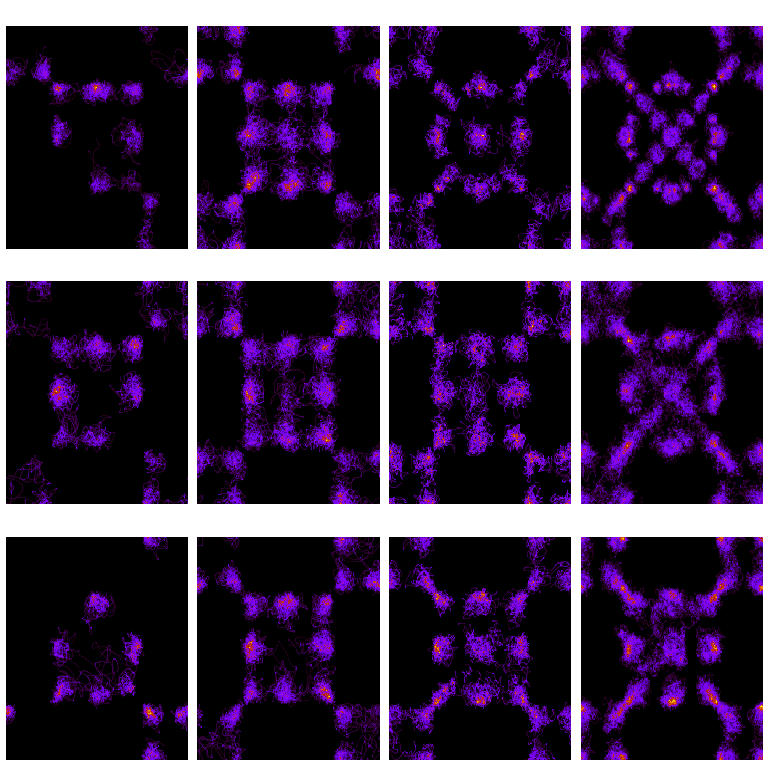
\includegraphics{zif8x-density}}%
    \gplfronttext
  \end{picture}%
\endgroup

    \caption{2D density maps of the adsorbed nitrogen atoms positions in the $xy$
    plane at various loadings in \ZIF8 (top), \ZIFCl (middle), and \ZIFBr
    (bottom). The loading increases from left to right.}
    \label{fig:fr:zif8x:density}
\end{figure}

\newpage
\section{Champs de force à partir de données \abinitio}

\begin{figure}[ht]
    \centering
    % GNUPLOT: LaTeX picture with Postscript
\begingroup
  \makeatletter
  \providecommand\color[2][]{%
    \GenericError{(gnuplot) \space\space\space\@spaces}{%
      Package color not loaded in conjunction with
      terminal option `colourtext'%
    }{See the gnuplot documentation for explanation.%
    }{Either use 'blacktext' in gnuplot or load the package
      color.sty in LaTeX.}%
    \renewcommand\color[2][]{}%
  }%
  \providecommand\includegraphics[2][]{%
    \GenericError{(gnuplot) \space\space\space\@spaces}{%
      Package graphicx or graphics not loaded%
    }{See the gnuplot documentation for explanation.%
    }{The gnuplot epslatex terminal needs graphicx.sty or graphics.sty.}%
    \renewcommand\includegraphics[2][]{}%
  }%
  \providecommand\rotatebox[2]{#2}%
  \@ifundefined{ifGPcolor}{%
    \newif\ifGPcolor
    \GPcolortrue
  }{}%
  \@ifundefined{ifGPblacktext}{%
    \newif\ifGPblacktext
    \GPblacktextfalse
  }{}%
  % define a \g@addto@macro without @ in the name:
  \let\gplgaddtomacro\g@addto@macro
  % define empty templates for all commands taking text:
  \gdef\gplbacktext{}%
  \gdef\gplfronttext{}%
  \makeatother
  \ifGPblacktext
    % no textcolor at all
    \def\colorrgb#1{}%
    \def\colorgray#1{}%
  \else
    % gray or color?
    \ifGPcolor
      \def\colorrgb#1{\color[rgb]{#1}}%
      \def\colorgray#1{\color[gray]{#1}}%
      \expandafter\def\csname LTw\endcsname{\color{white}}%
      \expandafter\def\csname LTb\endcsname{\color{black}}%
      \expandafter\def\csname LTa\endcsname{\color{black}}%
      \expandafter\def\csname LT0\endcsname{\color[rgb]{1,0,0}}%
      \expandafter\def\csname LT1\endcsname{\color[rgb]{0,1,0}}%
      \expandafter\def\csname LT2\endcsname{\color[rgb]{0,0,1}}%
      \expandafter\def\csname LT3\endcsname{\color[rgb]{1,0,1}}%
      \expandafter\def\csname LT4\endcsname{\color[rgb]{0,1,1}}%
      \expandafter\def\csname LT5\endcsname{\color[rgb]{1,1,0}}%
      \expandafter\def\csname LT6\endcsname{\color[rgb]{0,0,0}}%
      \expandafter\def\csname LT7\endcsname{\color[rgb]{1,0.3,0}}%
      \expandafter\def\csname LT8\endcsname{\color[rgb]{0.5,0.5,0.5}}%
    \else
      % gray
      \def\colorrgb#1{\color{black}}%
      \def\colorgray#1{\color[gray]{#1}}%
      \expandafter\def\csname LTw\endcsname{\color{white}}%
      \expandafter\def\csname LTb\endcsname{\color{black}}%
      \expandafter\def\csname LTa\endcsname{\color{black}}%
      \expandafter\def\csname LT0\endcsname{\color{black}}%
      \expandafter\def\csname LT1\endcsname{\color{black}}%
      \expandafter\def\csname LT2\endcsname{\color{black}}%
      \expandafter\def\csname LT3\endcsname{\color{black}}%
      \expandafter\def\csname LT4\endcsname{\color{black}}%
      \expandafter\def\csname LT5\endcsname{\color{black}}%
      \expandafter\def\csname LT6\endcsname{\color{black}}%
      \expandafter\def\csname LT7\endcsname{\color{black}}%
      \expandafter\def\csname LT8\endcsname{\color{black}}%
    \fi
  \fi
    \setlength{\unitlength}{0.0500bp}%
    \ifx\gptboxheight\undefined%
      \newlength{\gptboxheight}%
      \newlength{\gptboxwidth}%
      \newsavebox{\gptboxtext}%
    \fi%
    \setlength{\fboxrule}{0.5pt}%
    \setlength{\fboxsep}{1pt}%
\begin{picture}(6800.00,4520.00)%
    \gplgaddtomacro\gplbacktext{%
      \csname LTb\endcsname%%
      \put(470,2685){\makebox(0,0)[r]{\strut{}$1$}}%
      \csname LTb\endcsname%%
      \put(470,2994){\makebox(0,0)[r]{\strut{}$1.2$}}%
      \csname LTb\endcsname%%
      \put(470,3304){\makebox(0,0)[r]{\strut{}$1.4$}}%
      \csname LTb\endcsname%%
      \put(470,3613){\makebox(0,0)[r]{\strut{}$1.6$}}%
      \csname LTb\endcsname%%
      \put(470,3922){\makebox(0,0)[r]{\strut{}$1.8$}}%
      \csname LTb\endcsname%%
      \put(470,4231){\makebox(0,0)[r]{\strut{}$2$}}%
      \csname LTb\endcsname%%
      \put(545,2552){\makebox(0,0){\strut{}$1$}}%
      \csname LTb\endcsname%%
      \put(1023,2552){\makebox(0,0){\strut{}$1.2$}}%
      \csname LTb\endcsname%%
      \put(1501,2552){\makebox(0,0){\strut{}$1.4$}}%
      \csname LTb\endcsname%%
      \put(1979,2552){\makebox(0,0){\strut{}$1.6$}}%
      \csname LTb\endcsname%%
      \put(2457,2552){\makebox(0,0){\strut{}$1.8$}}%
      \csname LTb\endcsname%%
      \put(2935,2552){\makebox(0,0){\strut{}$2$}}%
      \csname LTb\endcsname%%
      \put(808,4131){\makebox(0,0)[l]{\strut{}(a)}}%
    }%
    \gplgaddtomacro\gplfronttext{%
      \csname LTb\endcsname%%
      \put(37,3535){\rotatebox{-270}{\makebox(0,0){\strut{}\footnotesize MOF-FF bond lengths ($\AA$)}}}%
      \csname LTb\endcsname%%
      \put(1859,2353){\makebox(0,0){\strut{}\footnotesize DFT bond lengths ($\AA$)}}%
      \csname LTb\endcsname%%
      \put(2918,3337){\makebox(0,0)[r]{\strut{}\ZIFBr}}%
      \csname LTb\endcsname%%
      \put(2918,3111){\makebox(0,0)[r]{\strut{}\ZIFCl}}%
      \csname LTb\endcsname%%
      \put(2918,2885){\makebox(0,0)[r]{\strut{}\ZIFCH3}}%
    }%
    \gplgaddtomacro\gplbacktext{%
      \csname LTb\endcsname%%
      \put(3870,2685){\makebox(0,0)[r]{\strut{}$100$}}%
      \csname LTb\endcsname%%
      \put(3870,3110){\makebox(0,0)[r]{\strut{}$110$}}%
      \csname LTb\endcsname%%
      \put(3870,3536){\makebox(0,0)[r]{\strut{}$120$}}%
      \csname LTb\endcsname%%
      \put(3870,3961){\makebox(0,0)[r]{\strut{}$130$}}%
      \csname LTb\endcsname%%
      \put(3870,4386){\makebox(0,0)[r]{\strut{}$140$}}%
      \csname LTb\endcsname%%
      \put(3945,2552){\makebox(0,0){\strut{}$100$}}%
      \csname LTb\endcsname%%
      \put(4602,2552){\makebox(0,0){\strut{}$110$}}%
      \csname LTb\endcsname%%
      \put(5260,2552){\makebox(0,0){\strut{}$120$}}%
      \csname LTb\endcsname%%
      \put(5917,2552){\makebox(0,0){\strut{}$130$}}%
      \csname LTb\endcsname%%
      \put(6574,2552){\makebox(0,0){\strut{}$140$}}%
      \csname LTb\endcsname%%
      \put(4208,4131){\makebox(0,0)[l]{\strut{}(b)}}%
    }%
    \gplgaddtomacro\gplfronttext{%
      \csname LTb\endcsname%%
      \put(3437,3535){\rotatebox{-270}{\makebox(0,0){\strut{}\footnotesize MOF-FF angles (°)}}}%
      \csname LTb\endcsname%%
      \put(5259,2353){\makebox(0,0){\strut{}\footnotesize DFT angles (°)}}%
    }%
    \gplgaddtomacro\gplbacktext{%
      \csname LTb\endcsname%%
      \put(545,425){\makebox(0,0)[r]{\strut{}$-200$}}%
      \csname LTb\endcsname%%
      \put(545,851){\makebox(0,0)[r]{\strut{}$-100$}}%
      \csname LTb\endcsname%%
      \put(545,1276){\makebox(0,0)[r]{\strut{}$0$}}%
      \csname LTb\endcsname%%
      \put(545,1702){\makebox(0,0)[r]{\strut{}$100$}}%
      \csname LTb\endcsname%%
      \put(545,2127){\makebox(0,0)[r]{\strut{}$200$}}%
      \csname LTb\endcsname%%
      \put(620,292){\makebox(0,0){\strut{}$-200$}}%
      \csname LTb\endcsname%%
      \put(1259,292){\makebox(0,0){\strut{}$-100$}}%
      \csname LTb\endcsname%%
      \put(1897,292){\makebox(0,0){\strut{}$0$}}%
      \csname LTb\endcsname%%
      \put(2536,292){\makebox(0,0){\strut{}$100$}}%
      \csname LTb\endcsname%%
      \put(3174,292){\makebox(0,0){\strut{}$200$}}%
      \csname LTb\endcsname%%
      \put(875,1872){\makebox(0,0)[l]{\strut{}(c)}}%
    }%
    \gplgaddtomacro\gplfronttext{%
      \csname LTb\endcsname%%
      \put(37,1276){\rotatebox{-270}{\makebox(0,0){\strut{}\footnotesize MOF-FF dihedral angles (°)}}}%
      \csname LTb\endcsname%%
      \put(1897,93){\makebox(0,0){\strut{}\footnotesize DFT dihedral angles (°)}}%
    }%
    \gplgaddtomacro\gplbacktext{%
      \csname LTb\endcsname%%
      \put(3945,425){\makebox(0,0)[r]{\strut{}$0$}}%
      \csname LTb\endcsname%%
      \put(3945,851){\makebox(0,0)[r]{\strut{}$500$}}%
      \csname LTb\endcsname%%
      \put(3945,1276){\makebox(0,0)[r]{\strut{}$1000$}}%
      \csname LTb\endcsname%%
      \put(3945,1702){\makebox(0,0)[r]{\strut{}$1500$}}%
      \csname LTb\endcsname%%
      \put(3945,2127){\makebox(0,0)[r]{\strut{}$2000$}}%
      \csname LTb\endcsname%%
      \put(4020,292){\makebox(0,0){\strut{}$0$}}%
      \csname LTb\endcsname%%
      \put(4659,292){\makebox(0,0){\strut{}$500$}}%
      \csname LTb\endcsname%%
      \put(5297,292){\makebox(0,0){\strut{}$1000$}}%
      \csname LTb\endcsname%%
      \put(5936,292){\makebox(0,0){\strut{}$1500$}}%
      \csname LTb\endcsname%%
      \put(6574,292){\makebox(0,0){\strut{}$2000$}}%
      \csname LTb\endcsname%%
      \put(4275,1872){\makebox(0,0)[l]{\strut{}(d)}}%
    }%
    \gplgaddtomacro\gplfronttext{%
      \csname LTb\endcsname%%
      \put(3437,1276){\rotatebox{-270}{\makebox(0,0){\strut{}\footnotesize MOF-FF vibrations (\si{cm^{-1}})}}}%
      \csname LTb\endcsname%%
      \put(5297,93){\makebox(0,0){\strut{}\footnotesize DFT vibrations (\si{cm^{-1}})}}%
    }%
    \gplbacktext
    \put(0,0){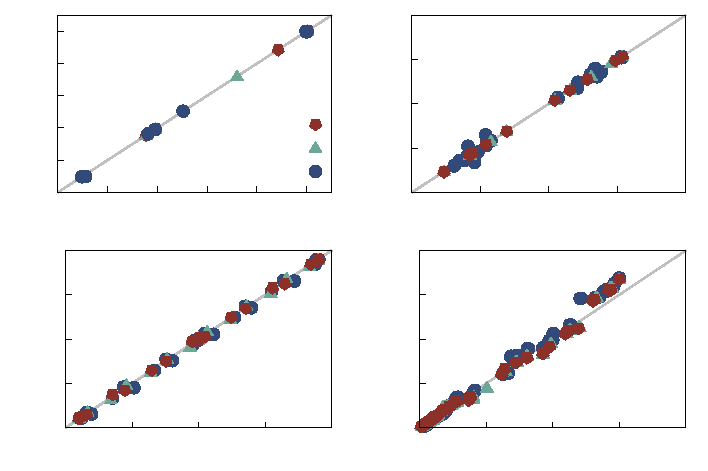
\includegraphics{mof-ff-validation}}%
    \gplfronttext
  \end{picture}%
\endgroup

    \caption{Comparisons of (a), (b) and (c): geometric parameters and (d):
    vibrational normal modes between the reference DFT data and the new MOF-FF
    force field.}
    \label{fig:fr:fig:mof-ff:validation}
\end{figure}

\newpage
\section{Intrusion d'électrolytes dans la \ZIF8}

\begin{figure}[ht]
    \centering
    % GNUPLOT: LaTeX picture with Postscript
\begingroup
  \makeatletter
  \providecommand\color[2][]{%
    \GenericError{(gnuplot) \space\space\space\@spaces}{%
      Package color not loaded in conjunction with
      terminal option `colourtext'%
    }{See the gnuplot documentation for explanation.%
    }{Either use 'blacktext' in gnuplot or load the package
      color.sty in LaTeX.}%
    \renewcommand\color[2][]{}%
  }%
  \providecommand\includegraphics[2][]{%
    \GenericError{(gnuplot) \space\space\space\@spaces}{%
      Package graphicx or graphics not loaded%
    }{See the gnuplot documentation for explanation.%
    }{The gnuplot epslatex terminal needs graphicx.sty or graphics.sty.}%
    \renewcommand\includegraphics[2][]{}%
  }%
  \providecommand\rotatebox[2]{#2}%
  \@ifundefined{ifGPcolor}{%
    \newif\ifGPcolor
    \GPcolortrue
  }{}%
  \@ifundefined{ifGPblacktext}{%
    \newif\ifGPblacktext
    \GPblacktextfalse
  }{}%
  % define a \g@addto@macro without @ in the name:
  \let\gplgaddtomacro\g@addto@macro
  % define empty templates for all commands taking text:
  \gdef\gplbacktext{}%
  \gdef\gplfronttext{}%
  \makeatother
  \ifGPblacktext
    % no textcolor at all
    \def\colorrgb#1{}%
    \def\colorgray#1{}%
  \else
    % gray or color?
    \ifGPcolor
      \def\colorrgb#1{\color[rgb]{#1}}%
      \def\colorgray#1{\color[gray]{#1}}%
      \expandafter\def\csname LTw\endcsname{\color{white}}%
      \expandafter\def\csname LTb\endcsname{\color{black}}%
      \expandafter\def\csname LTa\endcsname{\color{black}}%
      \expandafter\def\csname LT0\endcsname{\color[rgb]{1,0,0}}%
      \expandafter\def\csname LT1\endcsname{\color[rgb]{0,1,0}}%
      \expandafter\def\csname LT2\endcsname{\color[rgb]{0,0,1}}%
      \expandafter\def\csname LT3\endcsname{\color[rgb]{1,0,1}}%
      \expandafter\def\csname LT4\endcsname{\color[rgb]{0,1,1}}%
      \expandafter\def\csname LT5\endcsname{\color[rgb]{1,1,0}}%
      \expandafter\def\csname LT6\endcsname{\color[rgb]{0,0,0}}%
      \expandafter\def\csname LT7\endcsname{\color[rgb]{1,0.3,0}}%
      \expandafter\def\csname LT8\endcsname{\color[rgb]{0.5,0.5,0.5}}%
    \else
      % gray
      \def\colorrgb#1{\color{black}}%
      \def\colorgray#1{\color[gray]{#1}}%
      \expandafter\def\csname LTw\endcsname{\color{white}}%
      \expandafter\def\csname LTb\endcsname{\color{black}}%
      \expandafter\def\csname LTa\endcsname{\color{black}}%
      \expandafter\def\csname LT0\endcsname{\color{black}}%
      \expandafter\def\csname LT1\endcsname{\color{black}}%
      \expandafter\def\csname LT2\endcsname{\color{black}}%
      \expandafter\def\csname LT3\endcsname{\color{black}}%
      \expandafter\def\csname LT4\endcsname{\color{black}}%
      \expandafter\def\csname LT5\endcsname{\color{black}}%
      \expandafter\def\csname LT6\endcsname{\color{black}}%
      \expandafter\def\csname LT7\endcsname{\color{black}}%
      \expandafter\def\csname LT8\endcsname{\color{black}}%
    \fi
  \fi
    \setlength{\unitlength}{0.0500bp}%
    \ifx\gptboxheight\undefined%
      \newlength{\gptboxheight}%
      \newlength{\gptboxwidth}%
      \newsavebox{\gptboxtext}%
    \fi%
    \setlength{\fboxrule}{0.5pt}%
    \setlength{\fboxsep}{1pt}%
\begin{picture}(6800.00,3960.00)%
    \gplgaddtomacro\gplbacktext{%
      \csname LTb\endcsname%%
      \put(514,694){\makebox(0,0)[r]{\strut{}$0$}}%
      \csname LTb\endcsname%%
      \put(514,1456){\makebox(0,0)[r]{\strut{}$2$}}%
      \csname LTb\endcsname%%
      \put(514,2218){\makebox(0,0)[r]{\strut{}$4$}}%
      \csname LTb\endcsname%%
      \put(514,2980){\makebox(0,0)[r]{\strut{}$6$}}%
      \csname LTb\endcsname%%
      \put(514,3742){\makebox(0,0)[r]{\strut{}$8$}}%
      \csname LTb\endcsname%%
      \put(633,477){\makebox(0,0){\strut{}$0$}}%
      \csname LTb\endcsname%%
      \put(1996,477){\makebox(0,0){\strut{}$5$}}%
      \csname LTb\endcsname%%
      \put(3359,477){\makebox(0,0){\strut{}$10$}}%
      \csname LTb\endcsname%%
      \put(4722,477){\makebox(0,0){\strut{}$15$}}%
      \csname LTb\endcsname%%
      \put(6085,477){\makebox(0,0){\strut{}$20$}}%
      \csname LTb\endcsname%%
      \put(6204,694){\makebox(0,0)[l]{\strut{}$0$}}%
      \csname LTb\endcsname%%
      \put(6204,1456){\makebox(0,0)[l]{\strut{}$2$}}%
      \csname LTb\endcsname%%
      \put(6204,2218){\makebox(0,0)[l]{\strut{}$4$}}%
      \csname LTb\endcsname%%
      \put(6204,2980){\makebox(0,0)[l]{\strut{}$6$}}%
      \csname LTb\endcsname%%
      \put(6204,3742){\makebox(0,0)[l]{\strut{}$8$}}%
      \csname LTb\endcsname%%
      \put(3168,3171){\makebox(0,0)[l]{\strut{}Li-Cl neighbors}}%
    }%
    \gplgaddtomacro\gplfronttext{%
      \csname LTb\endcsname%%
      \put(178,2218){\rotatebox{-270}{\makebox(0,0){\strut{}Water neighbors}}}%
      \csname LTb\endcsname%%
      \put(3359,152){\makebox(0,0){\strut{}Concentration (mol/L)}}%
      \csname LTb\endcsname%%
      \put(2218,3547){\makebox(0,0)[r]{\strut{}water}}%
      \csname LTb\endcsname%%
      \put(3375,3547){\makebox(0,0)[r]{\strut{}Li}}%
      \csname LTb\endcsname%%
      \put(4532,3547){\makebox(0,0)[r]{\strut{}Cl}}%
    }%
    \gplbacktext
    \put(0,0){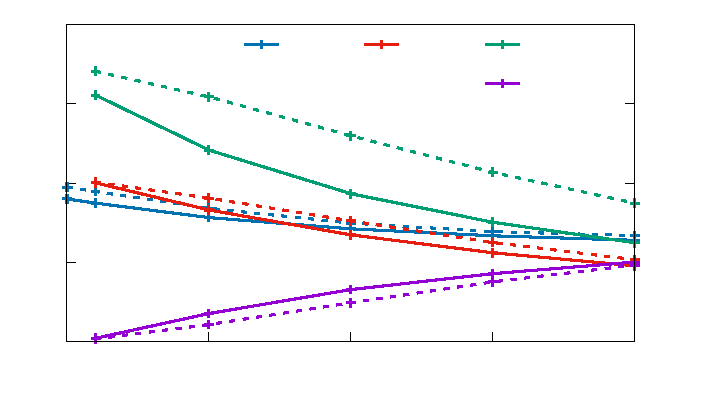
\includegraphics{licl-zif-neighbors}}%
    \gplfronttext
  \end{picture}%
\endgroup

    \caption{Number of water neighbors in the first solvation shell in the
    confined liquid (plain lines) and the bulk liquid (dotted lines) as
    function of the concentration, at the constant pressure of \SI{0}{GPa}.
    The number of chlorine neighbors for lithium ions is also represented.}
    \label{fig:licl-zif:neighbors}
\end{figure}

\begin{figure}[ht]
    \centering
    % GNUPLOT: LaTeX picture with Postscript
\begingroup
  \makeatletter
  \providecommand\color[2][]{%
    \GenericError{(gnuplot) \space\space\space\@spaces}{%
      Package color not loaded in conjunction with
      terminal option `colourtext'%
    }{See the gnuplot documentation for explanation.%
    }{Either use 'blacktext' in gnuplot or load the package
      color.sty in LaTeX.}%
    \renewcommand\color[2][]{}%
  }%
  \providecommand\includegraphics[2][]{%
    \GenericError{(gnuplot) \space\space\space\@spaces}{%
      Package graphicx or graphics not loaded%
    }{See the gnuplot documentation for explanation.%
    }{The gnuplot epslatex terminal needs graphicx.sty or graphics.sty.}%
    \renewcommand\includegraphics[2][]{}%
  }%
  \providecommand\rotatebox[2]{#2}%
  \@ifundefined{ifGPcolor}{%
    \newif\ifGPcolor
    \GPcolortrue
  }{}%
  \@ifundefined{ifGPblacktext}{%
    \newif\ifGPblacktext
    \GPblacktextfalse
  }{}%
  % define a \g@addto@macro without @ in the name:
  \let\gplgaddtomacro\g@addto@macro
  % define empty templates for all commands taking text:
  \gdef\gplbacktext{}%
  \gdef\gplfronttext{}%
  \makeatother
  \ifGPblacktext
    % no textcolor at all
    \def\colorrgb#1{}%
    \def\colorgray#1{}%
  \else
    % gray or color?
    \ifGPcolor
      \def\colorrgb#1{\color[rgb]{#1}}%
      \def\colorgray#1{\color[gray]{#1}}%
      \expandafter\def\csname LTw\endcsname{\color{white}}%
      \expandafter\def\csname LTb\endcsname{\color{black}}%
      \expandafter\def\csname LTa\endcsname{\color{black}}%
      \expandafter\def\csname LT0\endcsname{\color[rgb]{1,0,0}}%
      \expandafter\def\csname LT1\endcsname{\color[rgb]{0,1,0}}%
      \expandafter\def\csname LT2\endcsname{\color[rgb]{0,0,1}}%
      \expandafter\def\csname LT3\endcsname{\color[rgb]{1,0,1}}%
      \expandafter\def\csname LT4\endcsname{\color[rgb]{0,1,1}}%
      \expandafter\def\csname LT5\endcsname{\color[rgb]{1,1,0}}%
      \expandafter\def\csname LT6\endcsname{\color[rgb]{0,0,0}}%
      \expandafter\def\csname LT7\endcsname{\color[rgb]{1,0.3,0}}%
      \expandafter\def\csname LT8\endcsname{\color[rgb]{0.5,0.5,0.5}}%
    \else
      % gray
      \def\colorrgb#1{\color{black}}%
      \def\colorgray#1{\color[gray]{#1}}%
      \expandafter\def\csname LTw\endcsname{\color{white}}%
      \expandafter\def\csname LTb\endcsname{\color{black}}%
      \expandafter\def\csname LTa\endcsname{\color{black}}%
      \expandafter\def\csname LT0\endcsname{\color{black}}%
      \expandafter\def\csname LT1\endcsname{\color{black}}%
      \expandafter\def\csname LT2\endcsname{\color{black}}%
      \expandafter\def\csname LT3\endcsname{\color{black}}%
      \expandafter\def\csname LT4\endcsname{\color{black}}%
      \expandafter\def\csname LT5\endcsname{\color{black}}%
      \expandafter\def\csname LT6\endcsname{\color{black}}%
      \expandafter\def\csname LT7\endcsname{\color{black}}%
      \expandafter\def\csname LT8\endcsname{\color{black}}%
    \fi
  \fi
    \setlength{\unitlength}{0.0500bp}%
    \ifx\gptboxheight\undefined%
      \newlength{\gptboxheight}%
      \newlength{\gptboxwidth}%
      \newsavebox{\gptboxtext}%
    \fi%
    \setlength{\fboxrule}{0.5pt}%
    \setlength{\fboxsep}{1pt}%
\begin{picture}(7580.00,5100.00)%
    \gplgaddtomacro\gplbacktext{%
      \csname LTb\endcsname%%
      \put(408,2667){\makebox(0,0)[r]{\strut{}$0$}}%
      \csname LTb\endcsname%%
      \put(408,3037){\makebox(0,0)[r]{\strut{}$1$}}%
      \csname LTb\endcsname%%
      \put(408,3408){\makebox(0,0)[r]{\strut{}$2$}}%
      \csname LTb\endcsname%%
      \put(408,3778){\makebox(0,0)[r]{\strut{}$3$}}%
      \csname LTb\endcsname%%
      \put(408,4148){\makebox(0,0)[r]{\strut{}$4$}}%
      \csname LTb\endcsname%%
      \put(510,2481){\makebox(0,0){\strut{}$0$}}%
      \csname LTb\endcsname%%
      \put(1253,2481){\makebox(0,0){\strut{}$5$}}%
      \csname LTb\endcsname%%
      \put(1997,2481){\makebox(0,0){\strut{}$10$}}%
      \csname LTb\endcsname%%
      \put(2740,2481){\makebox(0,0){\strut{}$15$}}%
      \csname LTb\endcsname%%
      \put(3483,2481){\makebox(0,0){\strut{}$20$}}%
    }%
    \gplgaddtomacro\gplfronttext{%
      \csname LTb\endcsname%%
      \put(120,3407){\rotatebox{-270}{\makebox(0,0){\strut{}$\tau_1$ (ps)}}}%
      \csname LTb\endcsname%%
      \put(1137,4440){\makebox(0,0){\strut{}\footnotesize 0}}%
      \csname LTb\endcsname%%
      \put(1768,4440){\makebox(0,0){\strut{}\footnotesize 0.33}}%
      \csname LTb\endcsname%%
      \put(2399,4440){\makebox(0,0){\strut{}\footnotesize 0.67}}%
      \csname LTb\endcsname%%
      \put(3031,4440){\makebox(0,0){\strut{}\footnotesize 1}}%
      \csname LTb\endcsname%%
      \put(2084,5016){\makebox(0,0){\strut{}\footnotesize bulk liquid pressure (GPa)}}%
    }%
    \gplgaddtomacro\gplbacktext{%
      \csname LTb\endcsname%%
      \put(4198,2667){\makebox(0,0)[r]{\strut{}$0$}}%
      \csname LTb\endcsname%%
      \put(4198,3037){\makebox(0,0)[r]{\strut{}$25$}}%
      \csname LTb\endcsname%%
      \put(4198,3408){\makebox(0,0)[r]{\strut{}$50$}}%
      \csname LTb\endcsname%%
      \put(4198,3778){\makebox(0,0)[r]{\strut{}$75$}}%
      \csname LTb\endcsname%%
      \put(4198,4148){\makebox(0,0)[r]{\strut{}$100$}}%
      \csname LTb\endcsname%%
      \put(4300,2481){\makebox(0,0){\strut{}$0$}}%
      \csname LTb\endcsname%%
      \put(5043,2481){\makebox(0,0){\strut{}$5$}}%
      \csname LTb\endcsname%%
      \put(5787,2481){\makebox(0,0){\strut{}$10$}}%
      \csname LTb\endcsname%%
      \put(6530,2481){\makebox(0,0){\strut{}$15$}}%
      \csname LTb\endcsname%%
      \put(7273,2481){\makebox(0,0){\strut{}$20$}}%
    }%
    \gplgaddtomacro\gplfronttext{%
      \csname LTb\endcsname%%
      \put(3808,3407){\rotatebox{-270}{\makebox(0,0){\strut{}$\tau_2$ (ps)}}}%
    }%
    \gplgaddtomacro\gplbacktext{%
      \csname LTb\endcsname%%
      \put(408,627){\makebox(0,0)[r]{\strut{}$0$}}%
      \csname LTb\endcsname%%
      \put(408,998){\makebox(0,0)[r]{\strut{}$25$}}%
      \csname LTb\endcsname%%
      \put(408,1368){\makebox(0,0)[r]{\strut{}$50$}}%
      \csname LTb\endcsname%%
      \put(408,1739){\makebox(0,0)[r]{\strut{}$75$}}%
      \csname LTb\endcsname%%
      \put(408,2109){\makebox(0,0)[r]{\strut{}$100$}}%
      \csname LTb\endcsname%%
      \put(510,441){\makebox(0,0){\strut{}$0$}}%
      \csname LTb\endcsname%%
      \put(1253,441){\makebox(0,0){\strut{}$5$}}%
      \csname LTb\endcsname%%
      \put(1997,441){\makebox(0,0){\strut{}$10$}}%
      \csname LTb\endcsname%%
      \put(2740,441){\makebox(0,0){\strut{}$15$}}%
      \csname LTb\endcsname%%
      \put(3483,441){\makebox(0,0){\strut{}$20$}}%
    }%
    \gplgaddtomacro\gplfronttext{%
      \csname LTb\endcsname%%
      \put(69,1368){\rotatebox{-270}{\makebox(0,0){\strut{}$A_1$ (\%)}}}%
      \csname LTb\endcsname%%
      \put(1996,162){\makebox(0,0){\strut{}\footnotesize concentration (mol/L)}}%
    }%
    \gplgaddtomacro\gplbacktext{%
      \csname LTb\endcsname%%
      \put(4198,627){\makebox(0,0)[r]{\strut{}$0$}}%
      \csname LTb\endcsname%%
      \put(4198,998){\makebox(0,0)[r]{\strut{}$25$}}%
      \csname LTb\endcsname%%
      \put(4198,1368){\makebox(0,0)[r]{\strut{}$50$}}%
      \csname LTb\endcsname%%
      \put(4198,1739){\makebox(0,0)[r]{\strut{}$75$}}%
      \csname LTb\endcsname%%
      \put(4198,2109){\makebox(0,0)[r]{\strut{}$100$}}%
      \csname LTb\endcsname%%
      \put(4300,441){\makebox(0,0){\strut{}$0$}}%
      \csname LTb\endcsname%%
      \put(5043,441){\makebox(0,0){\strut{}$5$}}%
      \csname LTb\endcsname%%
      \put(5787,441){\makebox(0,0){\strut{}$10$}}%
      \csname LTb\endcsname%%
      \put(6530,441){\makebox(0,0){\strut{}$15$}}%
      \csname LTb\endcsname%%
      \put(7273,441){\makebox(0,0){\strut{}$20$}}%
    }%
    \gplgaddtomacro\gplfronttext{%
      \csname LTb\endcsname%%
      \put(3808,1368){\rotatebox{-270}{\makebox(0,0){\strut{}$A_2$ (\%)}}}%
      \csname LTb\endcsname%%
      \put(5786,162){\makebox(0,0){\strut{}\footnotesize concentration (mol/L)}}%
    }%
    \gplgaddtomacro\gplbacktext{%
    }%
    \gplgaddtomacro\gplfronttext{%
      \csname LTb\endcsname%%
      \put(4926,4440){\makebox(0,0){\strut{}\footnotesize 0}}%
      \csname LTb\endcsname%%
      \put(5557,4440){\makebox(0,0){\strut{}\footnotesize 0.33}}%
      \csname LTb\endcsname%%
      \put(6188,4440){\makebox(0,0){\strut{}\footnotesize 0.67}}%
      \csname LTb\endcsname%%
      \put(6820,4440){\makebox(0,0){\strut{}\footnotesize 1}}%
      \csname LTb\endcsname%%
      \put(5873,5016){\makebox(0,0){\strut{}\footnotesize confined liquid pressure (GPa)}}%
    }%
    \gplgaddtomacro\gplbacktext{%
    }%
    \gplgaddtomacro\gplfronttext{%
    }%
    \gplgaddtomacro\gplbacktext{%
    }%
    \gplgaddtomacro\gplfronttext{%
    }%
    \gplgaddtomacro\gplbacktext{%
    }%
    \gplgaddtomacro\gplfronttext{%
    }%
    \gplbacktext
    \put(0,0){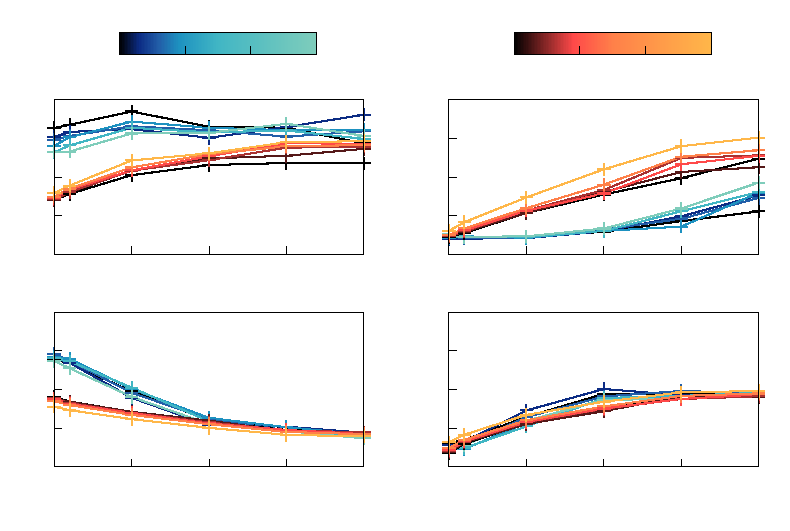
\includegraphics{licl-zif-hbonds-fit-pressure}}%
    \gplfronttext
  \end{picture}%
\endgroup

    \caption{Variations of the time constant and weights of the bi-exponential
    hydrogen bonds autocorrelation decay as function of the pressure in bulk
    (blue shades) and confined (red shades) liquids.}
    \label{fig:licl-zif:hbonds:fit:pressure}
\end{figure}

\begin{figure}[ht]
    \centering
    % GNUPLOT: LaTeX picture with Postscript
\begingroup
  \makeatletter
  \providecommand\color[2][]{%
    \GenericError{(gnuplot) \space\space\space\@spaces}{%
      Package color not loaded in conjunction with
      terminal option `colourtext'%
    }{See the gnuplot documentation for explanation.%
    }{Either use 'blacktext' in gnuplot or load the package
      color.sty in LaTeX.}%
    \renewcommand\color[2][]{}%
  }%
  \providecommand\includegraphics[2][]{%
    \GenericError{(gnuplot) \space\space\space\@spaces}{%
      Package graphicx or graphics not loaded%
    }{See the gnuplot documentation for explanation.%
    }{The gnuplot epslatex terminal needs graphicx.sty or graphics.sty.}%
    \renewcommand\includegraphics[2][]{}%
  }%
  \providecommand\rotatebox[2]{#2}%
  \@ifundefined{ifGPcolor}{%
    \newif\ifGPcolor
    \GPcolortrue
  }{}%
  \@ifundefined{ifGPblacktext}{%
    \newif\ifGPblacktext
    \GPblacktextfalse
  }{}%
  % define a \g@addto@macro without @ in the name:
  \let\gplgaddtomacro\g@addto@macro
  % define empty templates for all commands taking text:
  \gdef\gplbacktext{}%
  \gdef\gplfronttext{}%
  \makeatother
  \ifGPblacktext
    % no textcolor at all
    \def\colorrgb#1{}%
    \def\colorgray#1{}%
  \else
    % gray or color?
    \ifGPcolor
      \def\colorrgb#1{\color[rgb]{#1}}%
      \def\colorgray#1{\color[gray]{#1}}%
      \expandafter\def\csname LTw\endcsname{\color{white}}%
      \expandafter\def\csname LTb\endcsname{\color{black}}%
      \expandafter\def\csname LTa\endcsname{\color{black}}%
      \expandafter\def\csname LT0\endcsname{\color[rgb]{1,0,0}}%
      \expandafter\def\csname LT1\endcsname{\color[rgb]{0,1,0}}%
      \expandafter\def\csname LT2\endcsname{\color[rgb]{0,0,1}}%
      \expandafter\def\csname LT3\endcsname{\color[rgb]{1,0,1}}%
      \expandafter\def\csname LT4\endcsname{\color[rgb]{0,1,1}}%
      \expandafter\def\csname LT5\endcsname{\color[rgb]{1,1,0}}%
      \expandafter\def\csname LT6\endcsname{\color[rgb]{0,0,0}}%
      \expandafter\def\csname LT7\endcsname{\color[rgb]{1,0.3,0}}%
      \expandafter\def\csname LT8\endcsname{\color[rgb]{0.5,0.5,0.5}}%
    \else
      % gray
      \def\colorrgb#1{\color{black}}%
      \def\colorgray#1{\color[gray]{#1}}%
      \expandafter\def\csname LTw\endcsname{\color{white}}%
      \expandafter\def\csname LTb\endcsname{\color{black}}%
      \expandafter\def\csname LTa\endcsname{\color{black}}%
      \expandafter\def\csname LT0\endcsname{\color{black}}%
      \expandafter\def\csname LT1\endcsname{\color{black}}%
      \expandafter\def\csname LT2\endcsname{\color{black}}%
      \expandafter\def\csname LT3\endcsname{\color{black}}%
      \expandafter\def\csname LT4\endcsname{\color{black}}%
      \expandafter\def\csname LT5\endcsname{\color{black}}%
      \expandafter\def\csname LT6\endcsname{\color{black}}%
      \expandafter\def\csname LT7\endcsname{\color{black}}%
      \expandafter\def\csname LT8\endcsname{\color{black}}%
    \fi
  \fi
    \setlength{\unitlength}{0.0500bp}%
    \ifx\gptboxheight\undefined%
      \newlength{\gptboxheight}%
      \newlength{\gptboxwidth}%
      \newsavebox{\gptboxtext}%
    \fi%
    \setlength{\fboxrule}{0.5pt}%
    \setlength{\fboxsep}{1pt}%
\begin{picture}(5660.00,5660.00)%
    \gplgaddtomacro\gplbacktext{%
      \csname LTb\endcsname%%
      \put(752,3264){\makebox(0,0)[r]{\strut{}$-10$}}%
      \csname LTb\endcsname%%
      \put(752,3627){\makebox(0,0)[r]{\strut{}$0$}}%
      \csname LTb\endcsname%%
      \put(752,3990){\makebox(0,0)[r]{\strut{}$10$}}%
      \csname LTb\endcsname%%
      \put(752,4353){\makebox(0,0)[r]{\strut{}$20$}}%
      \csname LTb\endcsname%%
      \put(752,4716){\makebox(0,0)[r]{\strut{}$30$}}%
      \csname LTb\endcsname%%
      \put(752,5079){\makebox(0,0)[r]{\strut{}$40$}}%
      \csname LTb\endcsname%%
      \put(752,5442){\makebox(0,0)[r]{\strut{}$50$}}%
      \csname LTb\endcsname%%
      \put(871,3047){\makebox(0,0){\strut{}$-20$}}%
      \csname LTb\endcsname%%
      \put(1425,3047){\makebox(0,0){\strut{}$-15$}}%
      \csname LTb\endcsname%%
      \put(1979,3047){\makebox(0,0){\strut{}$-10$}}%
      \csname LTb\endcsname%%
      \put(2533,3047){\makebox(0,0){\strut{}$-5$}}%
      \csname LTb\endcsname%%
      \put(3087,3047){\makebox(0,0){\strut{}$0$}}%
      \csname LTb\endcsname%%
      \put(3640,3047){\makebox(0,0){\strut{}$5$}}%
      \csname LTb\endcsname%%
      \put(4194,3047){\makebox(0,0){\strut{}$10$}}%
      \csname LTb\endcsname%%
      \put(4748,3047){\makebox(0,0){\strut{}$15$}}%
      \csname LTb\endcsname%%
      \put(5302,3047){\makebox(0,0){\strut{}$20$}}%
    }%
    \gplgaddtomacro\gplfronttext{%
      \csname LTb\endcsname%%
      \put(178,4353){\rotatebox{-270}{\makebox(0,0){\strut{}free energy (kcal/mol)}}}%
      \csname LTb\endcsname%%
      \put(2924,5247){\makebox(0,0)[r]{\strut{}\ce{Li}}}%
      \csname LTb\endcsname%%
      \put(2924,5030){\makebox(0,0)[r]{\strut{}\ce{Cl}}}%
      \csname LTb\endcsname%%
      \put(2924,4813){\makebox(0,0)[r]{\strut{}\ce{H2O}}}%
    }%
    \gplgaddtomacro\gplbacktext{%
      \csname LTb\endcsname%%
      \put(633,694){\makebox(0,0)[r]{\strut{}$0$}}%
      \csname LTb\endcsname%%
      \put(633,1078){\makebox(0,0)[r]{\strut{}$2$}}%
      \csname LTb\endcsname%%
      \put(633,1462){\makebox(0,0)[r]{\strut{}$4$}}%
      \csname LTb\endcsname%%
      \put(633,1845){\makebox(0,0)[r]{\strut{}$6$}}%
      \csname LTb\endcsname%%
      \put(633,2229){\makebox(0,0)[r]{\strut{}$8$}}%
      \csname LTb\endcsname%%
      \put(633,2613){\makebox(0,0)[r]{\strut{}$10$}}%
      \csname LTb\endcsname%%
      \put(752,477){\makebox(0,0){\strut{}$-20$}}%
      \csname LTb\endcsname%%
      \put(1321,477){\makebox(0,0){\strut{}$-15$}}%
      \csname LTb\endcsname%%
      \put(1890,477){\makebox(0,0){\strut{}$-10$}}%
      \csname LTb\endcsname%%
      \put(2458,477){\makebox(0,0){\strut{}$-5$}}%
      \csname LTb\endcsname%%
      \put(3027,477){\makebox(0,0){\strut{}$0$}}%
      \csname LTb\endcsname%%
      \put(3596,477){\makebox(0,0){\strut{}$5$}}%
      \csname LTb\endcsname%%
      \put(4165,477){\makebox(0,0){\strut{}$10$}}%
      \csname LTb\endcsname%%
      \put(4733,477){\makebox(0,0){\strut{}$15$}}%
      \csname LTb\endcsname%%
      \put(5302,477){\makebox(0,0){\strut{}$20$}}%
    }%
    \gplgaddtomacro\gplfronttext{%
      \csname LTb\endcsname%%
      \put(178,1653){\rotatebox{-270}{\makebox(0,0){\strut{}number of neighbors}}}%
      \csname LTb\endcsname%%
      \put(3027,152){\makebox(0,0){\strut{}x ($\AA$)}}%
    }%
    \gplbacktext
    \put(0,0){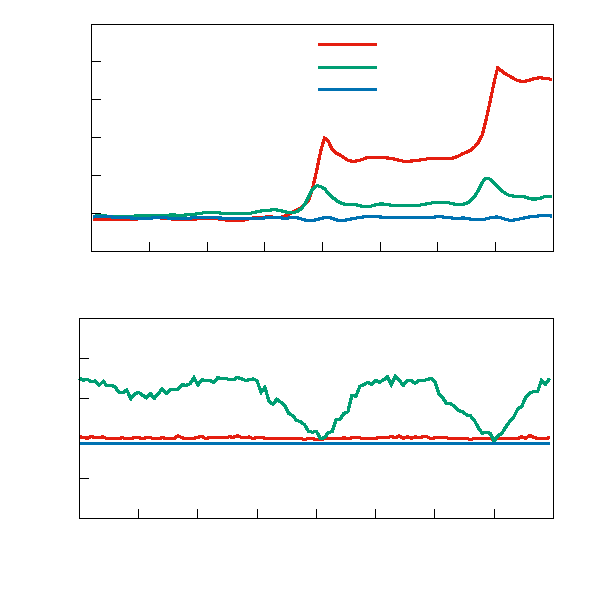
\includegraphics{licl-zif-free-energy}}%
    \gplfronttext
  \end{picture}%
\endgroup

    \caption{Free energy profile (top) of a single molecule entering \ZIF8 and
    corresponding number of neighbors (bottom) in the first solvation shell as
    function of the position of the molecule along the (111) crystallographic
    axis. The first \ZIF8 windows is at $x=0$; the $x<0$ area corresponds to
    bulk water, and the $x>0$ area to water-filled \ZIF8. We evaluated the
    uncertainty on the free energy profile using Monte Carlo
    bootstrapping\cite{WHAM}, and found it to be at most \SI{0.08}{kcal/mol} for
    \ce{H2O}, and \SI{0.3}{kcal/mol} for \ce{Cl-} and \ce{Li+}.}
    \label{fig:licl-zif:free}
\end{figure}

\newpage
\section{Adsorption d'eau dans les imogolites}


\ref{fig:imogolite:structure}

\begin{figure}[ht]
    \centering
    % GNUPLOT: LaTeX picture with Postscript
\begingroup
  \makeatletter
  \providecommand\color[2][]{%
    \GenericError{(gnuplot) \space\space\space\@spaces}{%
      Package color not loaded in conjunction with
      terminal option `colourtext'%
    }{See the gnuplot documentation for explanation.%
    }{Either use 'blacktext' in gnuplot or load the package
      color.sty in LaTeX.}%
    \renewcommand\color[2][]{}%
  }%
  \providecommand\includegraphics[2][]{%
    \GenericError{(gnuplot) \space\space\space\@spaces}{%
      Package graphicx or graphics not loaded%
    }{See the gnuplot documentation for explanation.%
    }{The gnuplot epslatex terminal needs graphicx.sty or graphics.sty.}%
    \renewcommand\includegraphics[2][]{}%
  }%
  \providecommand\rotatebox[2]{#2}%
  \@ifundefined{ifGPcolor}{%
    \newif\ifGPcolor
    \GPcolortrue
  }{}%
  \@ifundefined{ifGPblacktext}{%
    \newif\ifGPblacktext
    \GPblacktextfalse
  }{}%
  % define a \g@addto@macro without @ in the name:
  \let\gplgaddtomacro\g@addto@macro
  % define empty templates for all commands taking text:
  \gdef\gplbacktext{}%
  \gdef\gplfronttext{}%
  \makeatother
  \ifGPblacktext
    % no textcolor at all
    \def\colorrgb#1{}%
    \def\colorgray#1{}%
  \else
    % gray or color?
    \ifGPcolor
      \def\colorrgb#1{\color[rgb]{#1}}%
      \def\colorgray#1{\color[gray]{#1}}%
      \expandafter\def\csname LTw\endcsname{\color{white}}%
      \expandafter\def\csname LTb\endcsname{\color{black}}%
      \expandafter\def\csname LTa\endcsname{\color{black}}%
      \expandafter\def\csname LT0\endcsname{\color[rgb]{1,0,0}}%
      \expandafter\def\csname LT1\endcsname{\color[rgb]{0,1,0}}%
      \expandafter\def\csname LT2\endcsname{\color[rgb]{0,0,1}}%
      \expandafter\def\csname LT3\endcsname{\color[rgb]{1,0,1}}%
      \expandafter\def\csname LT4\endcsname{\color[rgb]{0,1,1}}%
      \expandafter\def\csname LT5\endcsname{\color[rgb]{1,1,0}}%
      \expandafter\def\csname LT6\endcsname{\color[rgb]{0,0,0}}%
      \expandafter\def\csname LT7\endcsname{\color[rgb]{1,0.3,0}}%
      \expandafter\def\csname LT8\endcsname{\color[rgb]{0.5,0.5,0.5}}%
    \else
      % gray
      \def\colorrgb#1{\color{black}}%
      \def\colorgray#1{\color[gray]{#1}}%
      \expandafter\def\csname LTw\endcsname{\color{white}}%
      \expandafter\def\csname LTb\endcsname{\color{black}}%
      \expandafter\def\csname LTa\endcsname{\color{black}}%
      \expandafter\def\csname LT0\endcsname{\color{black}}%
      \expandafter\def\csname LT1\endcsname{\color{black}}%
      \expandafter\def\csname LT2\endcsname{\color{black}}%
      \expandafter\def\csname LT3\endcsname{\color{black}}%
      \expandafter\def\csname LT4\endcsname{\color{black}}%
      \expandafter\def\csname LT5\endcsname{\color{black}}%
      \expandafter\def\csname LT6\endcsname{\color{black}}%
      \expandafter\def\csname LT7\endcsname{\color{black}}%
      \expandafter\def\csname LT8\endcsname{\color{black}}%
    \fi
  \fi
    \setlength{\unitlength}{0.0500bp}%
    \ifx\gptboxheight\undefined%
      \newlength{\gptboxheight}%
      \newlength{\gptboxwidth}%
      \newsavebox{\gptboxtext}%
    \fi%
    \setlength{\fboxrule}{0.5pt}%
    \setlength{\fboxsep}{1pt}%
\begin{picture}(7580.00,3680.00)%
    \gplgaddtomacro\gplbacktext{%
    }%
    \gplgaddtomacro\gplfronttext{%
      \csname LTb\endcsname%%
      \put(752,434){\makebox(0,0){\strut{}$-10$}}%
      \csname LTb\endcsname%%
      \put(1324,434){\makebox(0,0){\strut{}$-5$}}%
      \csname LTb\endcsname%%
      \put(1895,434){\makebox(0,0){\strut{}$0$}}%
      \csname LTb\endcsname%%
      \put(2466,434){\makebox(0,0){\strut{}$5$}}%
      \csname LTb\endcsname%%
      \put(3038,434){\makebox(0,0){\strut{}$10$}}%
      \csname LTb\endcsname%%
      \put(1895,109){\makebox(0,0){\strut{}$x\ (\AA)$}}%
      \csname LTb\endcsname%%
      \put(521,805){\makebox(0,0)[r]{\strut{}$-10$}}%
      \csname LTb\endcsname%%
      \put(521,1377){\makebox(0,0)[r]{\strut{}$-5$}}%
      \csname LTb\endcsname%%
      \put(521,1948){\makebox(0,0)[r]{\strut{}$0$}}%
      \csname LTb\endcsname%%
      \put(521,2519){\makebox(0,0)[r]{\strut{}$5$}}%
      \csname LTb\endcsname%%
      \put(521,3091){\makebox(0,0)[r]{\strut{}$10$}}%
      \csname LTb\endcsname%%
      \put(105,1948){\rotatebox{-270}{\makebox(0,0){\strut{}$y\ (\AA)$}}}%
    }%
    \gplgaddtomacro\gplbacktext{%
    }%
    \gplgaddtomacro\gplfronttext{%
      \csname LTb\endcsname%%
      \put(4542,434){\makebox(0,0){\strut{}$-10$}}%
      \csname LTb\endcsname%%
      \put(5114,434){\makebox(0,0){\strut{}$-5$}}%
      \csname LTb\endcsname%%
      \put(5685,434){\makebox(0,0){\strut{}$0$}}%
      \csname LTb\endcsname%%
      \put(6256,434){\makebox(0,0){\strut{}$5$}}%
      \csname LTb\endcsname%%
      \put(6828,434){\makebox(0,0){\strut{}$10$}}%
      \csname LTb\endcsname%%
      \put(5685,109){\makebox(0,0){\strut{}$x\ (\AA)$}}%
      \csname LTb\endcsname%%
      \put(4311,805){\makebox(0,0)[r]{\strut{}$-10$}}%
      \csname LTb\endcsname%%
      \put(4311,1377){\makebox(0,0)[r]{\strut{}$-5$}}%
      \csname LTb\endcsname%%
      \put(4311,1948){\makebox(0,0)[r]{\strut{}$0$}}%
      \csname LTb\endcsname%%
      \put(4311,2519){\makebox(0,0)[r]{\strut{}$5$}}%
      \csname LTb\endcsname%%
      \put(4311,3091){\makebox(0,0)[r]{\strut{}$10$}}%
      \csname LTb\endcsname%%
      \put(3895,1948){\rotatebox{-270}{\makebox(0,0){\strut{}$y\ (\AA)$}}}%
    }%
    \gplbacktext
    \put(0,0){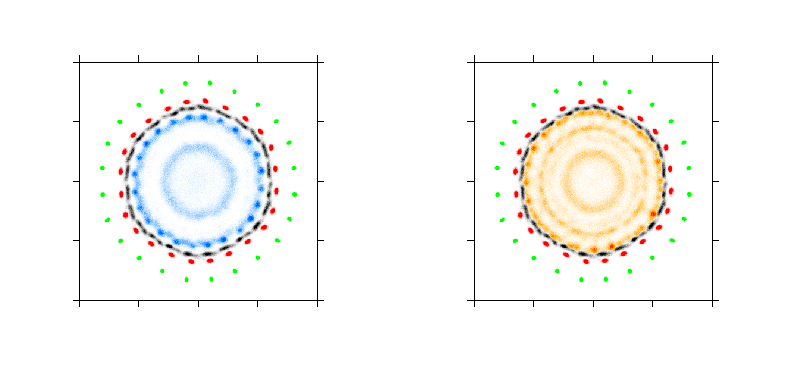
\includegraphics{imogolite-density-xy}}%
    \gplfronttext
  \end{picture}%
\endgroup

    \caption{Two-dimensional density profiles in the $xy$ plane for atoms from
    the silanol groups (Si in green, O in red, H in black) and water molecules
    (\ce{O_w} in blue and \ce{H_w} in orange).}
    \label{fig:imogolite:density:xy}
\end{figure}

\begin{figure}[ht]
    \centering
    % GNUPLOT: LaTeX picture with Postscript
\begingroup
  \makeatletter
  \providecommand\color[2][]{%
    \GenericError{(gnuplot) \space\space\space\@spaces}{%
      Package color not loaded in conjunction with
      terminal option `colourtext'%
    }{See the gnuplot documentation for explanation.%
    }{Either use 'blacktext' in gnuplot or load the package
      color.sty in LaTeX.}%
    \renewcommand\color[2][]{}%
  }%
  \providecommand\includegraphics[2][]{%
    \GenericError{(gnuplot) \space\space\space\@spaces}{%
      Package graphicx or graphics not loaded%
    }{See the gnuplot documentation for explanation.%
    }{The gnuplot epslatex terminal needs graphicx.sty or graphics.sty.}%
    \renewcommand\includegraphics[2][]{}%
  }%
  \providecommand\rotatebox[2]{#2}%
  \@ifundefined{ifGPcolor}{%
    \newif\ifGPcolor
    \GPcolortrue
  }{}%
  \@ifundefined{ifGPblacktext}{%
    \newif\ifGPblacktext
    \GPblacktextfalse
  }{}%
  % define a \g@addto@macro without @ in the name:
  \let\gplgaddtomacro\g@addto@macro
  % define empty templates for all commands taking text:
  \gdef\gplbacktext{}%
  \gdef\gplfronttext{}%
  \makeatother
  \ifGPblacktext
    % no textcolor at all
    \def\colorrgb#1{}%
    \def\colorgray#1{}%
  \else
    % gray or color?
    \ifGPcolor
      \def\colorrgb#1{\color[rgb]{#1}}%
      \def\colorgray#1{\color[gray]{#1}}%
      \expandafter\def\csname LTw\endcsname{\color{white}}%
      \expandafter\def\csname LTb\endcsname{\color{black}}%
      \expandafter\def\csname LTa\endcsname{\color{black}}%
      \expandafter\def\csname LT0\endcsname{\color[rgb]{1,0,0}}%
      \expandafter\def\csname LT1\endcsname{\color[rgb]{0,1,0}}%
      \expandafter\def\csname LT2\endcsname{\color[rgb]{0,0,1}}%
      \expandafter\def\csname LT3\endcsname{\color[rgb]{1,0,1}}%
      \expandafter\def\csname LT4\endcsname{\color[rgb]{0,1,1}}%
      \expandafter\def\csname LT5\endcsname{\color[rgb]{1,1,0}}%
      \expandafter\def\csname LT6\endcsname{\color[rgb]{0,0,0}}%
      \expandafter\def\csname LT7\endcsname{\color[rgb]{1,0.3,0}}%
      \expandafter\def\csname LT8\endcsname{\color[rgb]{0.5,0.5,0.5}}%
    \else
      % gray
      \def\colorrgb#1{\color{black}}%
      \def\colorgray#1{\color[gray]{#1}}%
      \expandafter\def\csname LTw\endcsname{\color{white}}%
      \expandafter\def\csname LTb\endcsname{\color{black}}%
      \expandafter\def\csname LTa\endcsname{\color{black}}%
      \expandafter\def\csname LT0\endcsname{\color{black}}%
      \expandafter\def\csname LT1\endcsname{\color{black}}%
      \expandafter\def\csname LT2\endcsname{\color{black}}%
      \expandafter\def\csname LT3\endcsname{\color{black}}%
      \expandafter\def\csname LT4\endcsname{\color{black}}%
      \expandafter\def\csname LT5\endcsname{\color{black}}%
      \expandafter\def\csname LT6\endcsname{\color{black}}%
      \expandafter\def\csname LT7\endcsname{\color{black}}%
      \expandafter\def\csname LT8\endcsname{\color{black}}%
    \fi
  \fi
    \setlength{\unitlength}{0.0500bp}%
    \ifx\gptboxheight\undefined%
      \newlength{\gptboxheight}%
      \newlength{\gptboxwidth}%
      \newsavebox{\gptboxtext}%
    \fi%
    \setlength{\fboxrule}{0.5pt}%
    \setlength{\fboxsep}{1pt}%
\begin{picture}(7360.00,7360.00)%
    \gplgaddtomacro\gplbacktext{%
    }%
    \gplgaddtomacro\gplfronttext{%
      \csname LTb\endcsname%%
      \put(1122,5142){\makebox(0,0){\strut{}$-10$}}%
      \csname LTb\endcsname%%
      \put(2380,5142){\makebox(0,0){\strut{}$-5$}}%
      \csname LTb\endcsname%%
      \put(3637,5142){\makebox(0,0){\strut{}$0$}}%
      \csname LTb\endcsname%%
      \put(4894,5142){\makebox(0,0){\strut{}$5$}}%
      \csname LTb\endcsname%%
      \put(6152,5142){\makebox(0,0){\strut{}$10$}}%
      \csname LTb\endcsname%%
      \put(693,5476){\makebox(0,0)[r]{\strut{}$-4.25$}}%
      \csname LTb\endcsname%%
      \put(693,6203){\makebox(0,0)[r]{\strut{}$0$}}%
      \csname LTb\endcsname%%
      \put(693,6930){\makebox(0,0)[r]{\strut{}$4.25$}}%
      \csname LTb\endcsname%%
      \put(277,6203){\rotatebox{-270}{\makebox(0,0){\strut{}$z$ (\AA)}}}%
    }%
    \gplgaddtomacro\gplbacktext{%
    }%
    \gplgaddtomacro\gplfronttext{%
      \csname LTb\endcsname%%
      \put(1122,2934){\makebox(0,0){\strut{}$-10$}}%
      \csname LTb\endcsname%%
      \put(2380,2934){\makebox(0,0){\strut{}$-5$}}%
      \csname LTb\endcsname%%
      \put(3637,2934){\makebox(0,0){\strut{}$0$}}%
      \csname LTb\endcsname%%
      \put(4894,2934){\makebox(0,0){\strut{}$5$}}%
      \csname LTb\endcsname%%
      \put(6152,2934){\makebox(0,0){\strut{}$10$}}%
      \csname LTb\endcsname%%
      \put(693,3268){\makebox(0,0)[r]{\strut{}$-4.25$}}%
      \csname LTb\endcsname%%
      \put(693,3995){\makebox(0,0)[r]{\strut{}$0$}}%
      \csname LTb\endcsname%%
      \put(693,4722){\makebox(0,0)[r]{\strut{}$4.25$}}%
      \csname LTb\endcsname%%
      \put(277,3995){\rotatebox{-270}{\makebox(0,0){\strut{}$z$ (\AA)}}}%
    }%
    \gplgaddtomacro\gplbacktext{%
    }%
    \gplgaddtomacro\gplfronttext{%
      \csname LTb\endcsname%%
      \put(1122,726){\makebox(0,0){\strut{}$-10$}}%
      \csname LTb\endcsname%%
      \put(2380,726){\makebox(0,0){\strut{}$-5$}}%
      \csname LTb\endcsname%%
      \put(3637,726){\makebox(0,0){\strut{}$0$}}%
      \csname LTb\endcsname%%
      \put(4894,726){\makebox(0,0){\strut{}$5$}}%
      \csname LTb\endcsname%%
      \put(6152,726){\makebox(0,0){\strut{}$10$}}%
      \csname LTb\endcsname%%
      \put(3637,401){\makebox(0,0){\strut{}circular coordinate (\AA)}}%
      \csname LTb\endcsname%%
      \put(693,1060){\makebox(0,0)[r]{\strut{}$-4.25$}}%
      \csname LTb\endcsname%%
      \put(693,1787){\makebox(0,0)[r]{\strut{}$0$}}%
      \csname LTb\endcsname%%
      \put(693,2514){\makebox(0,0)[r]{\strut{}$4.25$}}%
      \csname LTb\endcsname%%
      \put(277,1787){\rotatebox{-270}{\makebox(0,0){\strut{}$z$ (\AA)}}}%
    }%
    \gplbacktext
    \put(0,0){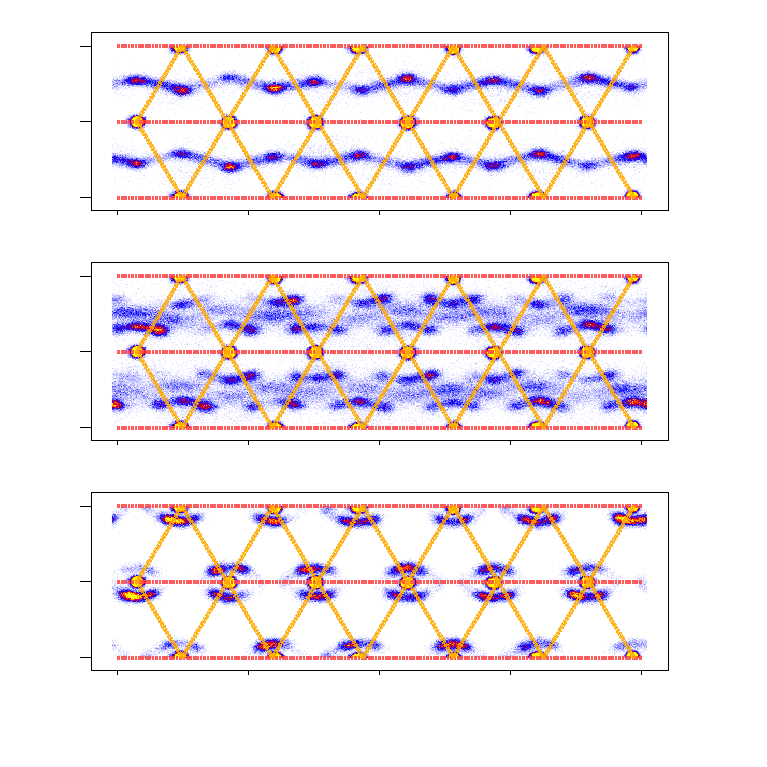
\includegraphics{imogolite-density-flat}}%
    \gplfronttext
  \end{picture}%
\endgroup

    \caption{Density profiles on the flattened hydrated nanotube planes for
    water oxygen (top) and water hydrogen (bottom). The circular coordinate
    corresponds to a curvilinear abscissa that draws a circle of radius $R =
    \SI{6.5}{\AA}$ centered on the axis $z$. On all the graphs, internal oxygen
    atoms appear as yellow dots.}
    \label{fig:imogolite:density:circular}
\end{figure}

\newpage
\section{Simulations hybride dans l'ensemble osmotique}

\newpage
\section*{Conclusions}

Les travaux présentés dans cette thèse portent sur l'étude de l'adsorption et de
l'intrusion dans les matériaux flexibles nanoporeux, la déformation de ces
matériaux et le couplage entre les deux phénomènes. Le confinement d'un fluide à
l'intérieur d'un réseau poreux a des effets significatifs sur ses propriétés
thermodynamiques, du fait de la compétition entre les interactions avec les
interfaces et les interactions avec le fluide même. Cette compétition génère de
nouveaux comportements, tels que de nouvelles phases fluides et des transitions
entre ces phases, et est particulièrement présente dans les matériaux
nanoporeux, où la largeur typique du pore et la distance typique des
interactions sont du même ordre de grandeur. D'autre part, la présence d'un
fluide confiné peut également avoir des effets importants sur le solide
environnant, créant de nouvelles phases et modifiant l'équilibre entre plusieurs
phases méta-stables. C'est particulièrement poignant dans le cas des matériaux
nanoporeux flexibles, tels que de nombreux MOFs.

Comme ces matériaux sont relativement récents, leur flexibilité a souvent été
négligée et ce n'est que ces dernières années que la communauté scientifique a
commencé à en tenir compte. Un exemple d'un tel changement est présenté dans la
première section de ce résumé, avec l'incorporation de l'ensemble osmotique dans
la théorie de la solution adsorbée idéale (IAST) pour l'étude de la
co-adsorption des gaz, menant à la création de la théorie dite \emph{Osmotic
Framework Adsorbed Solution Theory} (OFAST). J'ai pu démontré que IAST est
invalide \emph{par construction} pour le traitement de la co-adsorption lorsque
l'hôte adsorbant n'est pas inerte pendant l'adsorption. En particulier, j'ai
montré que IAST ne peut pas être utilisé pour la prédiction de la co-adsorption
de mélanges de fluides dans des matériaux présentant un comportement d'ouverture
de porte, et qu'il prédit une sélectivité non physique, jusqu'à deux ordres de
grandeur supérieurs à celle prédite par OFAST. Même lorsque IAST n'est pas
explicitement utilisé pour calculer la sélectivité dans matériaux flexibles, il
faut rester prudents en lorsque l'on compare des isothermes de corps purs en
présence de flexibilité. Les différences de pression d'ouverture des isothermes
peuvent conduire à des allégations de forte sélectivité, lorsque l'on applique
des concepts qui ne sont valables que pour des matrices hôtes rigides.

Il faut aussi veiller à ne pas aller trop loin dans l'autre sens, et attribuer
tous les comportements observés à la flexibilité des matériaux. Dans la
quatrième section de ce résumé, j'ai utilisé des simulations de dynamique
moléculaire \abinitio pour expliquer l'origine d'une isotherme étagé pour
l'adsorption d'azote dans \ZIFCH3 et \ZIFCl, et son absence dans la structure
similaire \ZIFBr. J'ai montré que si le réseau se déforme pendant l'adsorption
pour \ZIFCH3 et \ZIFCl, les déformations ne changent pas le volume accessible et
la distribution des pores de ces matériaux. Au lieu de cela, l'augmentation de
l'absorption dans l'isotherme est liée à une réorganisation du fluide confiné
dans les pores, réorganisation qui ne se produit pas dans \ZIFBr en raison de la
différence de taille des pores. Il est donc fondamental de tenir compte à la
fois des effets de flexibilité et de confinement lors de l'étude de l'adsorption
dans les matériaux nanoporeux flexibles.

Il en va de même pour l'intrusion, cousin de l'adsorption. Dans les section 4 et
5, j'ai utilisé des simulations moléculaires classiques pour étudier le
confinement sous haute pression de l'eau et de solutions d'électrolytes dans des
nanotubes d'imogolite et dans la \ZIF8. J'ai observé des effets de confinement
allant d'une organisation spatiale plus marquée, à des changements dans les
propriétés élastiques, et le ralentissement de la dynamique de l'eau. Il est
intéressant de noter que la présence d'ions à de forte concentrations peut avoir
les mêmes effets sur l'eau non confinée; structurant le réseau de liaisons
hydrogène et ralentissant la dynamique. L'intrusion de solution aqueuses dans un
matériau hydrophobe est un moyen prometteur de stocker et de dissiper l'énergie
mécanique. Il est possible d'ajuster le comportement et même de transformer un
système stockant de l'énergie à un système dissipatif d'énergie à la dissipation
en ajoutant des ions dans la solution aqueuses utilisée pour l'intrusion. J'ai
examiné l'impact des ions sur le comportement d'intrusion en utilisant des
simulations \emph{umbrella sampling} pour extraire le profil d'énergie libre
d'entrée dans la \ZIF8, montrant que les différents ions ont des barrières
différentes quand ils traversent les fenêtres de la \ZIF8. Cette étude est l'une
des premières sur le thème de l'intrusion d'électrolytes dans les MOF, et a
permis de mettre en lumière les comportements complexes qui émergent dans ces
systèmes.

La nécessité de tenir compte simultanément de l'adsorption et des déformations a
été un thème récurrent de toutes ces études. Mais les méthodes actuelles de
simulation ne permettent d'aborder qu'une seule dimension du problème: les
simulations de dynamique moléculaire peuvent décrire des déformations, mais la
modélisation de systèmes ouverts et donc l'adsorption n'est pas possible. Les
simulations de Monte-Carlo Metropolis peuvent être utilisées pour des systèmes
ouverts, mais elles ont du mal à échantillonner efficacement les déformations
collectives. Les simulations Monte-Carlo hybride sont une réponse possible à ce
dilemme, combinant l'efficacité de la dynamique moléculaire avec la polyvalence
des simulations Monte-Carlo (en particulier la possibilité d'échantillonner des
ensembles ouverts). Mon dernier section présente la méthode de simulation
Monte-Carlo hybride et son utilisation pour les simulations directes dans
l'ensemble osmotique. Pour accroître la portée de ces nouvelles méthodes au sein
de la communauté scientifique, il faut qu'elles soient facilement accessibles
sous forme de logiciels génériques, faciles à utiliser et efficaces.

Il y a une autre condition à remplir avant de pouvoir utiliser largement les
simulations d'ensembles osmotiques pour l'étude de l'adsorption et de
l'intrusion dans les cristaux nanoporeux flexibles: il nous faut pouvoir
calculer l'énergie liés à la flexibilité des matériaux et à leurs interactions
avec les fluides. Les méthodes premier principe ou \abinitio (comme la théorie
de la fonctionnelle de la densité) permettent de calculer avec précision
l'énergie de systèmes atomistiques arbitraires. Ces méthodes nécessitent
malheureusement une grande puissance de calcul, ce qui les empêche d'être
utilisés en routine sur de grands systèmes. Face à des systèmes d'une telle
taille --- que ce soit en termes de nombre d'atomes, d'échelle de temps des
processus ou de criblage à haut débit --- nous avons donc souvent recours aux
champs de force classiques.

Les champs de force classiques sont soit \emph{précis}, c'est-à-dire qu'ils
reproduisent bien la surface d'énergie potentielle réelle, soit
\emph{transférables}, c'est-à-dire utilisables avec plusieurs systèmes
différents. Les champs de forces transférables actuels ne sont pas bien adaptés
pour décrire la flexibilité résultant des liaisons de coordination, il faut donc
créer de nouveaux champs de forces pour ces systèmes. Historiquement, la
paramétrisation de nouveaux champs de forces a été un processus assez long et
fastidieux. Depuis quelques années, de nouvelles techniques basées sur
l'apprentissage statistique ou \emph{Machine Learning} ont été mises au point
pour la dérivation constante et rapide de champs de force précis. Je présente
une de ces techniques dans la troisème section de ce résumé, que j'ai utilisée
pour obtenir des champs de force pour la \ZIF8 et certains de ses dérivés à
partir de données \abinitio. Ces techniques automatiques sont particulièrement
cruciales pour l'étude des MOFs en raison de la grande diversité de leurs
structures. J'espère que la disponibilité de champs de force précis et de
logiciels offrant des simulations de Monte-Carlo hybride facilitera
l'utilisation de simulations moléculaires pour concevoir de nouveaux matériaux
adaptés à des applications spécifiques.

\begin{center}
    \pgfornament[width=6cm,color=CTsemi]{88}
\end{center}

Ces travaux ouvrent des perspectives dans plusieurs directions. En ce qui
concerne les méthodes de simulation moléculaire, le Monte-Carlo hybride semble
être une technique puissante, utilisable avec une grande variété de systèmes.
Tout d'abord, la méthode Monte-Carlo hybride étant basée sur la théorie des
chaines de Markov et le critère de Metropolis convergera toujours vers la
distribution dans l'espace des phases de l'ensemble statistique voulu. Au
contraire, la dynamique moléculaire échantillonne par défaut l'ensemble
microcanonique, et doit s'appuyer sur des thermostats et des barostats pour
échantillonner d'autres ensembles. Ces thermostats et surtout les barostats ne
sont pas tous égaux, et seuls certains algorithmes sont capables de générer
précisément l'ensemble souhaité. En même temps, les mouvements hybrides
améliorent grandement l'efficacité des simulations Monte-Carlo en tenant compte
de la courbure locale de la surface d'énergie potentielle.

Savoir s'il est possible de simuler des systèmes ouverts avec la dynamique
moléculaire reste aujourd'hui encore une question de recherche ouverte.
Inversement, de telles simulations sont couramment réalisées dans le cadre du
Monte-Carlo Grand Canonique. Le Monte-Carlo hybride pourrait ainsi être utilisé
pour la simulation d'ensembles ouverts et de systèmes dilués, tels que les
simulations à pH constant, la description de l'environnement ionique des
protéines ou la simulation de défauts dans les matériaux cristallins; améliorant
l'efficacité des ces simulations par rapport au Monte-Carlo classique et
permettant la simulation d'ensemble ouverts aux utilisateurs de dynamique
moléculaire. Grâce au critère d'acceptation de Metropolis, il n'est pas
nécessaire que la dynamique moléculaire courte utilisée par les mouvements
hybrides échantillonne un ensemble thermodynamique réel ou même un Hamiltonien
ayant un sens physique.  Cette propriété pourrait être exploitée pour créer des
simulations Monte-Carlo encore plus efficaces, par exemple en insérant
progressivement de nouvelles molécules dans un système tout en relaxant son
environnement.

Une autre perspective concerne les champs de forces classiques et leur capacité
à reproduire avec précision les surfaces énergétiques potentielles. L'approche
traditionnelle lors de la création de champs de force a été de décomposer
l'énergie en une somme de termes dépendant de valeurs scalaires simples avec une
signification physique: distances, longueur de liaison, angles et angles
dihèdres, \etc  Ces valeurs scalaires sont ensuite combinées dans des
expressions mathématiques simples, par exemple des fonctions puissance ou
exponentielles. Dans cette approche la surface d'énergie potentielle ne peut pas
inclure d'effets à trois corps ou plus, ni reproduire avec précision la forme de
la surfaces d'énergie potentielle de référence. Les outils d'apprentissage
statistique, en particulier les réseaux neuronaux et les processus gaussiens,
peuvent apporter des améliorations à ces deux problèmes. Premièrement, la
capacité des réseaux de neurones à reproduire des fonctions arbitraires de
$\mathds{R}^n$ à $\mathds{R}$ peut réduire l'écart entre les surfaces d'énergie
potentielle de référence et du champ de force. Par exemple, au lieu d'imposer un
potentiel de Lennard-Jones, les réseaux neuronaux peuvent reproduire les
variations exacte de l'énergie. Deuxièmement, les algorithmes d'apprentissage
statistique peuvent être couplés à de meilleurs descripteurs de la structure
atomique, tenant compte des effets à plusieurs corps. Dans dernières années, de
multiples équipes scientifiques indépendantes ont travaillé à la conception,
l'entrainement et l'évaluation de ces champs de forces basé sur l'apprentissage
statistique et des descripteurs associés. A ma connaissance, ces méthodes n'ont
pas encore été utilisées pour l'étude de matériaux nanoporeux flexibles.

\vfill
\begin{center}
    \pgfornament[width=6cm,color=CTsemi]{75}
\end{center}
\vfill\vfill

\end{otherlanguage}

\OnlyInSubfile{\printglobalbibliography}

\end{document}
